\documentclass[11pt]{article}
\usepackage[T1]{fontenc}
\usepackage{amsmath,amssymb,amsthm}
\usepackage[margin=1in]{geometry}
\usepackage{booktabs}
\usepackage{tikz}
\usetikzlibrary{positioning}
\usepackage{hyperref}

% ===== theorem environments =====
\theoremstyle{plain}
\newtheorem{theorem}{Theorem}[section]
\newtheorem{lemma}[theorem]{Lemma}
\newtheorem{proposition}[theorem]{Proposition}
\newtheorem{corollary}[theorem]{Corollary}
\newtheorem{conjecture}[theorem]{Conjecture}
\theoremstyle{definition}
\newtheorem{definition}[theorem]{Definition}
\newtheorem{remark}[theorem]{Remark}

% ===== macros =====
\newcommand{\N}{\mathbb{N}}
\newcommand{\rays}{S}
\newcommand{\rch}{r}
\newcommand{\Vk}{V_{k}}
\newcommand{\Dk}{D_{k}}
\newcommand{\DkD}{D_{k}^{\Delta}}
\newcommand{\DkS}{D_{k}^{\Sigma}}
\newcommand{\Mcut}{M_{\mathrm{cut}}}
\newcommand{\lam}{\lambda_{\mathrm{int}}}
\newcommand{\tstar}{t^{\ast}}
\newcommand{\wells}{\mathrm{wells}}
\newcommand{\dd}{\mathrm{d}}

\title{Sinks in the levels of the Goldbach re-pairing digraph:\\
a mod-3 valve, extremal-ray bridges, and a $\{2,3\}$ oscillation}
\author{F.~Gaudin\thanks{Universit\'e de Caen Normandie, France.
Email: \href{mailto:frederic.gaudin@unicaen.fr}{\texttt{frederic.gaudin@unicaen.fr}}.}}
\date{November 2026}

\begin{document}
\maketitle
\begin{NoHyper}
\begingroup
\renewcommand{\thefootnote}{}
\footnotetext{2020 \emph{Mathematics Subject Classification}:
11P32 (primary), 11N35, 11N36, 05C20, 11B13.}
\footnotetext{\emph{Keywords}: Goldbach partitions, prime pairs,
directed graph, singular series, mod-3 obstruction, sinks,
Hardy--Littlewood model.}
\endgroup
\end{NoHyper}

\begin{abstract}
For an integer $m \ge 4$, let $S(m) = \{t \ge 1 : m-t \text{ and }
m+t \text{ are prime}\}$ and $r(m) = |S(m)|$ (OEIS A061357). The
\emph{Goldbach re-pairing digraph} on $\{m \ge 4\}$ has an arc
$m \to n$ ($n \neq m$) whenever two elements $a < b$ of $S(m)$
yield a \emph{difference arc} to $n = m \mp (b-a)/2$ or a
\emph{sum arc} to $n = m \mp (a+b)/2$; the arc is \emph{descending}
if $n < m$, and \emph{retained} at level $k$ if $n < m$ and
$r(n) \ge k$. A \emph{$k$-well} ($k$-sink) is a vertex of
$V_k = \{m \ge 4 : r(m) \ge k\}$ emitting no retained arc.

We prove unconditionally: (i) a \emph{mod-3 valve}: no descending
arc goes from $m \not\equiv 0 \pmod 3$ to $n \equiv 0 \pmod 3$,
whereas every prime $p \ge 5$ admits infinitely many descending arcs
into $0 \pmod p$; (ii) a \emph{unique crossing mechanism}: descending
arcs between $1 \pmod 3$ and $2 \pmod 3$ arise solely from the
extremal ray $m-3$, present if and only if $2m-3$ is prime; (iii)
\emph{well-count certificates} on the residue-class minima modulo~$3$
of $V_k$, together with downward finiteness of each level; (iv) a
\emph{prime-quadruple characterisation} of descending adjacency;
and (v) \emph{local Schnirelmann coverage}: every dyadic interval
$[X,2X]$ ($X \ge X_0$) contains a vertex $m$ whose descending
difference arcs cover at least $c_1 m$ integers below $m$ ($c_1 > 0$
absolute).

Exhaustive verification for $m \le 10^6$ gives $2$ or $3$ wells on
$V_k \cap [4,10^6]$ for all $3 \le k \le 14\,089$, zero non-minimal
wells among $999\,947$ tested vertices, and perpetual windowed
oscillation between $2$ and $3$ wells. We formulate three main
conjectures governing the global well count, prime-quadruple
bottlenecks at gaps divisible by $6$, and the asymptotic density of
three-well levels.
\end{abstract}

\section{Introduction}

\subsection{Motivation}

For an integer $m \ge 4$, $\rch(m)$ counts the off-diagonal
representations $2m = p+q$ with $p < q$ both prime: this is the
sequence A061357 of the OEIS~\cite{oeis} (convention $t \ge 1$; the
diagonal pair $p = q = m$ for prime $m$ is excluded). The
distribution of $\rch(m)$ is conjecturally governed by the
Hardy--Littlewood singular series.

The \emph{re-pairing digraph} records how a representation of $2n$
can be drawn inside the partners of $2m$: two rays $a < b$ of $m$
produce children at distance $(b-a)/2$ and $(a+b)/2$ below (and
above) $m$. The object is autonomous: its definition uses no
unproved hypothesis; only the \emph{thickness} of its levels
$\Vk = \{m \ge 4 : \rch(m) \ge k\}$ involves the unproved
distribution law. Neighbouring graphs exist in the literature (the
factorisation graphs of Bo\.zek~\cite{bozek} (a static graph per
even integer, via addition and multiplication) and the oriented
bipartite graphs of Das--Ghosh--Ghosh--Sen~\cite{das} (connectivity
equivalent to the Goldbach conjecture)), but they are static
objects, with no dynamics internal to the representations
themselves.

The question of this paper is: \emph{does the descent inside $\Vk$
always terminate, and into how many wells?} A \emph{well} is a state
$m \in \Vk$ at which re-pairing produces no child rich enough to
remain in the level. The threshold
$L_k = \sup\{m \ge 4 : \rch(m) < k\}$ (with the convention
$\sup\varnothing = 3$; the last non-$k$-rich integer, an
A000954-type quantity~\cite{oeis}) governs the answer: under its
finiteness, the counting of wells reduces to a finite segment
(Proposition~\ref{prop:mcut}).

\subsection{What is proved, measured, conditional, open}
\label{sec:honest}

The proved part is unconditional and local or structural: the mod-3
valve (Theorem~\ref{thm:valve}), the $2m-3$ bridge
(Theorem~\ref{thm:bridge}), the descending arcs into $0$ at every
modulus $p \ge 5$ (Proposition~\ref{thm:pgates}), the descent ceiling
(Lemma~\ref{lem:ceiling}), the well certificates
(Theorems~\ref{thm:cert2} and~\ref{thm:cert3}), the bottleneck
bijection (Theorem~\ref{thm:bij}) and the trivial bound
(Lemma~\ref{lem:bound}). The dense $\Delta$-coverage of a rich
vertex (Theorem~\ref{thm:dense}) is unconditional; its sieve
inputs \eqref{eq:HA}--\eqref{eq:HC} in Section~\ref{sec:dense} are
discharged inside the proof via Halberstam--Richert~\cite[Theorem~5.7]{hr}
and an elementary local-factor bound; its combinatorial skeleton is
kernel-verified in the Lean artefact (Appendix~\ref{app:lean}). All
\emph{global} bounds ($|\wells(\Dk)| \le 3$ on the whole of $\N$)
follow \emph{unconditionally} from the margin conjecture
(Conjecture~\ref{conj:M}, Proposition~\ref{prop:master}); the
finiteness of $L_k$ (which already at $k = 1$ is the Goldbach
conjecture, hence unattainable by a finite bound) is invoked only
to reduce a fixed level to a finite segment (Corollary~\ref{cor:H}).
The measurements are finite-window computation data, never proofs.
The asymptotic regime (growth of $\rch$, prime tuples in linear
configuration) is covered in the literature
(Granville~\cite{granville}; Green--Tao~\cite{greentao}): the
present object is new only at finite scale, a limitation we state
explicitly.

\noindent\emph{Outline.} Section~\ref{sec:defs} gives the
definitions;
Section~\ref{sec:mod3} the mod-3 mechanism and the well
certificates (the autonomous theorems); Section~\ref{sec:bij} the
bottleneck bijection and bounds; Section~\ref{sec:mcut} the finite
reduction; Section~\ref{sec:data} the exhaustive data;
Section~\ref{sec:osc} the $\{2,3\}$ oscillation and dense
$\Delta$-coverage; Section~\ref{sec:conj} the conjectures and
models; Section~\ref{sec:fals} falsifiability and positioning;
Appendix~\ref{app:proto} the computation protocol;
Appendix~\ref{app:lean} the Lean artefact.

\section{Definitions and notation}
\label{sec:defs}

Throughout the paper, for real numbers $\alpha \le \beta$, interval
notation such as $[\alpha,\beta]$, $[\alpha,\beta)$, or
$(\alpha,\beta]$ denotes the corresponding set of integers
$[\alpha,\beta] \cap \mathbb{Z}$, $[\alpha,\beta) \cap \mathbb{Z}$,
or $(\alpha,\beta] \cap \mathbb{Z}$, unless real intervals are
explicitly indicated by context (as in integration domains or
continuous parameter ranges). For a finite set $A$, $|A|$ denotes
its cardinality, and $\mathbf{1}_{\{P\}}$ denotes the indicator
equal to $1$ when the predicate $P$ holds and $0$ otherwise. Let
$\mathbb{P}$ denote the set of prime numbers.

We also fix the standard Hardy--Littlewood twin-prime and
prime-quadruple constants via their convergent Euler products:
\[
C_2 \;=\; \prod_{\ell \ge 3} \frac{\ell(\ell - 2)}{(\ell - 1)^{2}}
 \;\approx\; 0.6601618,
\qquad
C_4 \;=\; \frac{27}{2} \prod_{\ell \ge 5}
 \frac{\ell^{3}(\ell - 4)}{(\ell - 1)^{4}}
 \;\approx\; 4.15118086,
\]
where $\ell$ runs over primes, together with the binary Goldbach
singular series for $m \ge 4$:
\[
\mathfrak{S}_2(2m)
 \;=\; 2 C_2 \prod_{\substack{\ell \ge 3 \\ \ell \mid m}}
 \frac{\ell - 1}{\ell - 2}
 \;=\; \prod_{\ell \ge 2} \mathrm{loc}_2(\ell; m),
\]
with local factors $\mathrm{loc}_2(2;m) = 2$ and
$\mathrm{loc}_2(\ell;m) = \ell(\ell - \nu_{2,\ell}(m))/(\ell-1)^{2}$
for $\ell \ge 3$, where
$\nu_{2,\ell}(m) = |\{m, -m\} \bmod \ell| \in \{1,2\}$.

\begin{definition}[rays, richness]\label{def:rays}
For $m \ge 4$ let
\[
\rays(m) = \{\,t \ge 1 : m-t \ \text{and}\ m+t \ \text{are both prime}\,\},
\qquad \rch(m) = |\rays(m)|.
\]
The elements of $\rays(m)$ are the \emph{rays} of $m$; $\rch(m)$ is
its \emph{richness} (OEIS A061357~\cite{oeis}, convention $t \ge 1$:
pairs $p < q$ of distinct primes; control values
$\rch(17) = \rch(23) = 3$). Equivalently $\rays(m)$ enumerates the
representations $2m = p + q$, $p < q$ prime, via $t = (q-p)/2$. The
\emph{partner set} is
\[
\mathrm{Part}(m)
 = \{\,p \in \mathbb{P} : 2m-p \in \mathbb{P},\ p \neq m\,\}
 = \{\,m - t : t \in \rays(m)\,\} \cup \{\,m + t : t \in \rays(m)\,\}.
\]
Every ray satisfies $1 \le t \le m-3$ and has parity opposite to $m$
(both partners are odd primes).
\end{definition}

\begin{definition}[children, arcs, retained arcs]\label{def:children}
For $a < b$ in $\rays(m)$, the pair \emph{re-pairs} around the four
\emph{children}
\[
n \in \bigl\{\, m - \tfrac{b-a}{2},\ m + \tfrac{b-a}{2},\
                 m - \tfrac{a+b}{2},\ m + \tfrac{a+b}{2}\,\bigr\}.
\]
An \emph{arc} $m \to n$ exists whenever $n \neq m$ is a child; it is
\emph{descending} when $n < m$. We write $C^{-}(m)$ for the set of
descending children of $m$, decomposed into the \emph{difference
children} $C_\Delta^{-}(m) = \{m - (b-a)/2 : a < b \text{ in }
\rays(m)\}$ and the \emph{sum children}
$C_\Sigma^{-}(m) = \{m - (a+b)/2 : a < b \text{ in } \rays(m)\}$, so
that $C^{-}(m) = C_\Delta^{-}(m) \cup C_\Sigma^{-}(m)$. A descending
child carries a re-paired prime pair: $n = m - (b-a)/2$ carries
$(m-b,\ m+a)$, and $n = m - (a+b)/2$ carries $(m-b,\ m-a)$, immediate
identities; in each case $2n$ is a sum of two distinct members of
$\mathrm{Part}(m)$, whence $n \ge 4$ and $\rch(n) \ge 1$. At level
$k$, an arc $m \to n$ is \emph{retained} when it is descending and
$\rch(n) \ge k$.
\end{definition}

\begin{remark}[$\Delta$-arcs versus $\Sigma$-arcs]\label{rem:dsarc}
The two descending children of a pair $a < b$ in $\rays(m)$ play
different geometric roles. Since $1 \le a < b \le m - 3$ share
the parity opposite to $m$ (so $a \ge 2$ when $m$ is odd), the
\emph{difference arc} lands at
\[
n_\Delta \;=\; m - \tfrac{b-a}{2} \;\in\;
\bigl[\lceil m/2 \rceil + 2,\ m - 1\bigr]
\]
and carries the re-paired primes $(m - b,\ m + a)$, one below and
one above $m$; the \emph{sum arc} lands at
\[
n_\Sigma \;=\; m - \tfrac{a+b}{2} \;\in\; [\,4,\ m - 3\,]
\]
and carries $(m - b,\ m - a)$, both below $m$. A $\Delta$-arc can
only reach the upper half $n > m/2$ of the predecessors, while a
$\Sigma$-arc may land anywhere in $[4, m-3]$; the two ascending
children $m + (b \pm a)/2$ complete the pair orbit. The
sub-digraphs $\DkD$ and $\DkS$ on $\Vk$, retaining only
$\Delta$-arcs (respectively, only $\Sigma$-arcs), refine
$\Dk = \DkD \cup \DkS$; the oscillation is entirely borne by
$\Delta$-arcs (Proposition~\ref{prop:sigmabridge}).
\end{remark}

\begin{definition}[levels, wells, fibres, class minima]
\label{def:levels}
For any directed graph $G = (V(G), E(G))$, let
$\wells(G) = \{m \in V(G) : \text{there is no } n \in V(G)
\text{ with } (m \to n) \in E(G)\}$ denote its set of sinks.
For $k \ge 1$, let $\Vk = \{m \ge 4 : \rch(m) \ge k\}$, and let
$\Dk$ be the directed graph on vertex set $\Vk$ whose arcs are the
retained descending arcs $m \to n$ ($n \in C^{-}(m) \cap \Vk$). A
\emph{$k$-well} ($k$-sink) is an element of $\wells(\Dk)$; we write
\[
a(k) \;=\; |\wells(\Dk)|,
\qquad
a^{\mathrm{win}}(k) \;=\; \bigl|\wells\bigl(\Dk[\Vk \cap [4,10^{6}]]\bigr)\bigr|,
\]
where $\Dk[U]$ denotes the sub-digraph of $\Dk$ induced by a subset
$U \subseteq \Vk$ (note that since every retained arc descends,
$\wells(\Dk[\Vk \cap [4,N]]) = \wells(\Dk) \cap [4,N]$ for every
$N \ge 4$). A well of $\Dk$ is \emph{interior} if it is not the
minimum of its residue class modulo~$3$ inside $\Vk$. The
\emph{neutral fibre} is $\Vk \cap \{m \equiv 0 \pmod 3\}$; the
\emph{charged fibres} are $\Vk \cap \{m \equiv c \pmod 3\}$,
$c \in \{1,2\}$. The \emph{class minima} are
\[
\mu_c(k) = \min \bigl(\Vk \cap \{\,m \equiv c \pmod 3\,\}\bigr),
\qquad c \in \{0,1,2\}
\]
(each fibre is nonempty, Lemma~\ref{lem:fibres}). We further write
$\mu_{\min}(k) = \min(\mu_1(k),\mu_2(k))$ and
$\mu_{\max}(k) = \max(\mu_1(k),\mu_2(k))$ for the extreme charged
minima; $\mu_{\max}(k)$ is a \emph{vertex}, not to be confused with
the child-richness cap $M(m)$ of Definition~\ref{def:margin}.
\end{definition}

\begin{definition}[extremal ray, bridge]\label{def:bridge}
The \emph{extremal ray} is $\tstar(m) = m-3$, the largest possible
ray; $\tstar(m) \in \rays(m)$ if and only if $2m-3$ is prime. For a
charged $m$ ($m \not\equiv 0 \pmod 3$), the \emph{bridge} is the
family of pairs $(a,\tstar(m))$ with
$a \in \rays(m) \setminus \{\tstar(m)\}$: the bridge is \emph{alive}
when $2m-3$ is prime and \emph{dead} otherwise. We call it the
\emph{$2m-3$ bridge}.
\end{definition}

\begin{definition}[bottleneck pair, witness count, HL4 model]
\label{def:bottleneck}
A \emph{bottleneck pair} $(u_1,u_2,k,c)$ consists of two vertices
$6 \le u_1 < u_2$ in a residue class $c \in \{0,1,2\}$ whose
common level $k = \min(\rch(u_1),\rch(u_2))$ exceeds the richness
of every other class-$c$ vertex in $[6, u_2)$:
\[
k \;>\; \max\{\,\rch(w) : 6 \le w < u_2,\ w \neq u_1,\ w \equiv c
   \pmod 3\,\},
\]
the maximum of an empty set being $0$ (so the first two
class-$c$ record vertices already satisfy the strict
inequality, e.g.\ $(u_1,u_2) = (6,9)$). Starting the range at
$m \ge 6$ omits the charged class starters $\{4,5\}$, thereby
excluding the degenerate challenger $(u_1,u_2) = (4,7)$ where
$\rch(u_2) = 1$ admits no ray pair $a < b$. The earlier
vertex $u_1$ is the \emph{leader} (the running class-$c$ record
on $[6, u_2)$) and $u_2$ the \emph{challenger} (it need not exceed
$\rch(u_1)$ itself, only every other vertex in the range). The
bottleneck is \emph{dead-bridge} when $2u_2 - 3$ is composite (for
charged $c \in \{1,2\}$, the descending children of $u_2$ are then
confined to class $c$, Corollary~\ref{cor:dead}; for neutral
$c = 0$, $u_2 > u_1 \ge 6$ forces $u_2 \ge 9$, so
$3 \mid 2u_2 - 3$ is automatically composite). For any integers
$4 \le u_1 < u_2$, writing $v = u_2 - u_1$, the \emph{witness count}
is, in the arity-$2$ form of a midpoint richness over the partner
set of $u_2$,
\begin{equation}\label{eq:arity2}
N(u_1,u_2)
 \;=\; r_{\mathrm{Part}(u_2)}(u_1)
 \;:=\; \bigl|\bigl\{\, \{p,q\} \subset \mathrm{Part}(u_2) :\
   p \neq q,\ \tfrac{p+q}{2} = u_1 \,\bigr\}\bigr|,
\end{equation}
where $r_A(m)$ counts the unordered pairs of $A$ whose midpoint
is $m$. Expanding the pair $\{p,q\}$, $p < q$, gives the explicit
quadruple form
\[
N(u_1,u_2) = \bigl|\{\,p \in \mathbb{P},\ 3 \le p \le u_1 - 1 :
   p,\ p + 2v,\ 2u_1 - p,\ 2u_2 - p \ \text{all prime},\
   p \neq 2u_1 - u_2 \,\}\bigr|,
\]
in which the two guards are presentation artefacts of the
expansion: an unordered pair $\{p,q\} \subset \mathrm{Part}(u_2)$
with midpoint $u_1$ already forces $p < u_1 < q = 2u_1 - p$, and
$u_2 \notin \mathrm{Part}(u_2)$ makes the exclusion
$q \neq u_2 \iff p \neq 2u_1 - u_2$ automatic. On a bottleneck pair
($u_1 \equiv u_2 \pmod 3$, hence $3 \mid v$), the Hardy--Littlewood
quadruple model predicts
$N(u_1,u_2) \approx \lam(u_1,u_2)
= \mathfrak{S}_4^{\mathrm{bn}}(u_1,u_2)\,J(u_1,u_2)$, where
\begin{align*}
J(u_1,u_2) &\;=\; \int_{3}^{\,u_1 - 1}
\frac{\dd x}
{\ln x\;\ln(x + 2v)\;\ln(2u_1 - x)\;\ln(2u_2 - x)},\\[1ex]
\mathfrak{S}_4^{\mathrm{bn}}(u_1,u_2) &\;=\;
2^{\mathbf{1}_{\{3 \mid u_2\}}}\, C_4
\prod_{\substack{\ell \ge 5\\
\ell \mid u_1 u_2 v (2u_2 - u_1)}}
\frac{\ell - \nu_\ell}{\ell - 4},
\end{align*}
with $J(u_1,u_2)$ evaluated over the real interval $[3, u_1-1]$ by
fine quadrature (not its asymptotic equivalent), and where
$\nu_\ell = |\{\,0,\, -2v,\, 2u_1,\, 2u_2\,\} \bmod \ell|$ counts
the distinct roots of the quadruple modulo $\ell$; the displayed
formula for $\mathfrak{S}_4^{\mathrm{bn}}$ uses $3 \mid v$ (i.e.\
$u_1 \equiv u_2 \pmod 3$, which holds at every bottleneck pair),
giving the $\ell = 3$ factor $2^{\mathbf{1}_{\{3 \mid u_2\}}}$. The
$951$ bottleneck records include neutral-class pairs ($3 \mid u_2$,
prefactor $2C_4$); the $674$ dead-bridge bottlenecks split into
$358$ charged and $316$ neutral pairs (a neutral $u_2$ is
automatically dead-bridge since $3 \mid 2u_2 - 3$).
\end{definition}

\begin{definition}[margin]\label{def:margin}
For $m \ge 4$ let
$M(m) = \max\{\,\rch(n) : n \in C^{-}(m)\,\}$
(with $M(m) = -\infty$ when $C^{-}(m) = \varnothing$),
$\tau(m) = \min\bigl(\rch(m),\, R(m)\bigr)$, where
$R(m) = \max\{\,\rch(w) : 4 \le w < m,\ w \equiv m \pmod 3\,\}$
is the running maximum of the richness in the mod-3 class of $m$
(an empty set gives $R(m) = 0$, only for the class starters
$m \in \{4, 5, 6\}$, which hence have $\tau = 0$; the range starts
at $4$ to include the class starters, unlike bottlenecks which
start at $6$), and define the
\emph{margin} $\delta(m) = M(m) - \tau(m)$. A vertex $m$ is an
interior well at level $k \ge 1$ if and only if
$M(m) < k \le \tau(m)$ (hence at some level $k \ge 1$ if and only if
$\tau(m) \ge 1$ and $\delta(m) < 0$). A vertex with
$\tau(m) \ge 2$ is called a \emph{vital vertex}: vital vertices
are exactly the
vertices eligible to be interior wells at some level $k \ge 2$.
\end{definition}

\begin{definition}[thresholds]\label{def:thresholds}
Let $L_k = \sup\{m \ge 4 : \rch(m) < k\}$ (with the convention
$\sup\varnothing = 3$) denote the last non-$k$-rich integer; note that
$\rch(4) = 1$ forces $L_k \ge 4$ for every $k \ge 2$. The
\emph{tail hypothesis} $H(k)$ asserts $L_k < \infty$. We write
$m_1(k) = \min \Vk$. For $k \ge 2$ and $L \ge 4$,
\[
\Mcut(k,L) = L + 1 + \Bigl\lfloor \frac{L - 4}{2k - 3} \Bigr\rfloor .
\]
\end{definition}

\begin{lemma}[every residue class is unboundedly rich]
\label{lem:fibres}
For each $c \in \{0,1,2\}$,
$\limsup_{m \equiv c \pmod 3} \rch(m) = +\infty$; in particular each
fibre of $\Vk$ is nonempty and $\mu_c(k) < \infty$ for every $k \ge 1$.
\end{lemma}

\begin{proof}
By the prime number theorem in arithmetic progressions, each
nonzero class modulo~$3$ contains $\gg X/\ln X$ primes up to $X$.
Pairing primes $p,q \equiv 1 \pmod 3$ (for $c = 1$),
$p,q \equiv 2 \pmod 3$ (for $c = 2$), respectively
$p \equiv 1 \pmod 3$, $q \equiv 2 \pmod 3$ (for $c = 0$), gives
$\gg X^{2}/\ln^{2} X$ pairs whose midpoint $(p+q)/2 \equiv c \pmod 3$
lies in $[4,X]$; the pigeonhole principle then yields a midpoint
$m \equiv c \pmod 3$ with $\rch(m) \gg X/\ln^{2} X$, unbounded as
$X \to \infty$.
\end{proof}

\section{The mod-3 mechanism}
\label{sec:mod3}

Everything in this section is unconditional (ZFC) and, except for
the certificates' measured regime, fully structural; the main
statements are formally verified in Lean~4
(Appendix~\ref{app:lean}).

\begin{lemma}[ray classes modulo $3$]\label{lem:ray3}
Let $m \ge 4$.
\begin{enumerate}
\item If $m \not\equiv 0 \pmod 3$ then no ray satisfies
      $t \equiv -m \pmod 3$, and a ray with $t \equiv m \pmod 3$ is
      necessarily the extremal ray $t = m - 3$ (so $2m-3$ is prime).
      Hence every ray of a charged vertex is either
      $\equiv 0 \pmod 3$ or extremal.
\item If $m \equiv 0 \pmod 3$ then no ray satisfies
      $t \equiv 0 \pmod 3$.
\end{enumerate}
\end{lemma}

\begin{proof}
If $t \equiv -m \pmod 3$ then $m + t \equiv 0 \pmod 3$ with
$m + t > 3$, so $m + t$ is composite: no such ray exists. If
$t \equiv m \pmod 3$ then $m - t \equiv 0 \pmod 3$; for $m - t$ to be
prime one needs $m - t = 3$, i.e.\ $t = m - 3$, and then
$m + t = 2m - 3$ must be prime. If $m \equiv 0 \pmod 3$ and
$t \equiv 0 \pmod 3$, both $m - t$ and $m + t$ are multiples of $3$;
$m + t > 3$ is composite, and $m - t = 3$ forces $t = m - 3$, whence
$m + t = 2m - 3 \equiv 0 \pmod 3$, composite for $m > 3$.
\end{proof}

\begin{theorem}[the mod-3 valve]\label{thm:valve}
No descending arc goes from a charged vertex to a neutral vertex:
for $m \not\equiv 0 \pmod 3$, every descending child $n \in C^{-}(m)$
satisfies $n \equiv m \pmod 3$ or $n \equiv 2m \pmod 3$, never
$n \equiv 0 \pmod 3$. Consequently each charged fibre is closed
under descent, while the neutral fibre \emph{leaks}: every ray pair
$a < b$ of a neutral parent emits one neutral and one charged
descending child (via its $\Sigma$-child when $a \equiv b \pmod 3$
and via its $\Delta$-child when $a \equiv -b \pmod 3$; no extremal
ray exists for $3 \mid m$, since $2m - 3 \equiv 0 \pmod 3$ is then
composite). Figure~\ref{fig:valve} summarises the descending-arc
rules.
\end{theorem}

\begin{proof}
Let $m$ be charged. By Lemma~\ref{lem:ray3} every ray of $m$ is
regular ($\equiv 0 \pmod 3$) or extremal ($= m-3 \equiv m \pmod 3$).
A pair of regular rays $a,b \equiv 0 \pmod 3$ gives children
$n = m - (b \pm a)/2 \equiv m \pmod 3$: the same charged class. A
pair $(a, m-3)$ with $a \equiv 0 \pmod 3$ gives the two descending
children $n = m - (m - 3 \mp a)/2 = (m \pm a + 3)/2$; since
$2n = m \pm a + 3 \equiv m \pmod 3$, both satisfy
$n \equiv 2m \pmod 3$ (the opposite charged class), while the two
ascending children $(3m - 3 \pm a)/2 \equiv 0 \pmod 3$ are $> m$,
hence not descending. No descending child is neutral. For a neutral
$m$, rays are never $\equiv 0 \pmod 3$; a pair
$a \equiv b \not\equiv 0 \pmod 3$ gives $(b-a)/2 \equiv 0 \pmod 3$
($\Delta$-child stays neutral) and
$(a+b)/2 \equiv a \not\equiv 0 \pmod 3$ ($\Sigma$-child is charged),
while $a \equiv -b \pmod 3$ gives $(a+b)/2 \equiv 0 \pmod 3$
($\Sigma$-child stays neutral) and
$(b-a)/2 \equiv -a \not\equiv 0 \pmod 3$ ($\Delta$-child is
charged): in either case a charged descending child occurs.
\end{proof}

\begin{theorem}[the $2m-3$ bridge]\label{thm:bridge}
A charged vertex $m$ emits a descending arc into the \emph{opposite}
charged class if and only if $2m-3$ is prime and $\rch(m) \ge 2$. In
that case the crossing children are exactly the descendants of the
extremal pairs $(a, m-3)$, $a \in \rays(m)$ regular:
\[
n_1 = \frac{m + a + 3}{2}, \qquad n_2 = \frac{m - a + 3}{2},
\]
carrying the re-paired pairs $2n_1 = 3 + (m + a)$ and
$2n_2 = 3 + (m - a)$.
\end{theorem}

\begin{proof}
By Lemma~\ref{lem:ray3}, pairs of regular rays keep the child in the
class of $m$; the only pairs able to leave it involve a ray
$\equiv m \pmod 3$, which is necessarily the extremal ray
$m-3$ (present if and only if $2m-3$ is prime), paired with at
least one regular ray $a \in \rays(m) \setminus \{m-3\}$, which
exists if and only if $\rch(m) \ge 2$ once $m-3 \in \rays(m)$
(e.g.\ at $m \in \{4,5,7\}$, $2m-3$ is prime yet $\rch(m) = 1$, so
no arc is emitted). The two descending children of $(a, m-3)$ are
$m - (m-3-a)/2 = (m+a+3)/2$ and $m - (m-3+a)/2 = (m-a+3)/2$,
re-pairing $(m-(m-3), m+a) = (3, m+a)$ and $(3, m-a)$ respectively.
\end{proof}

\begin{corollary}[dead bridge confines]\label{cor:dead}
If $m$ is charged and $2m-3$ is composite, every descending child of
$m$ lies in the same residue class as $m$ modulo~$3$.
\end{corollary}

\begin{proof}
Immediate from Theorems~\ref{thm:valve} and~\ref{thm:bridge}.
\end{proof}

\begin{figure}[htbp]
\centering
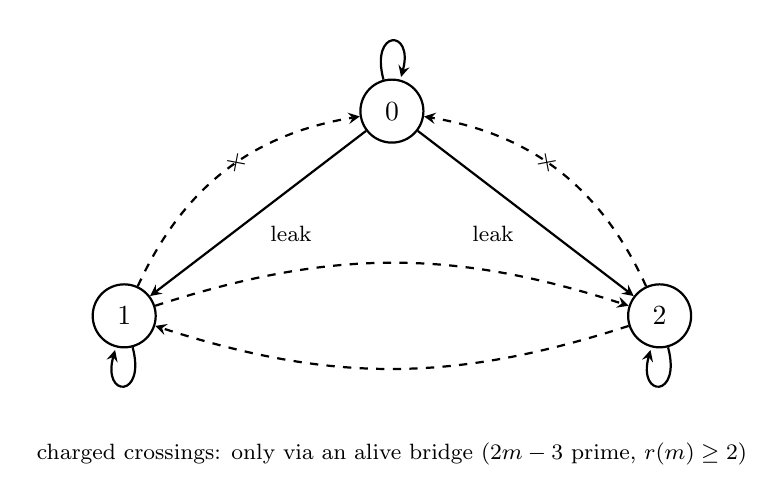
\begin{tikzpicture}[>=stealth, thick,
   cls/.style={circle,draw,minimum size=8mm,inner sep=1pt}]
\node[cls] (c0) at (0,2.6) {$0$};
\node[cls] (c1) at (-3.4,0) {$1$};
\node[cls] (c2) at (3.4,0) {$2$};
% self loops: intra-class descent always possible
\draw[->] (c0) edge[loop above] (c0);
\draw[->] (c1) edge[loop below] (c1);
\draw[->] (c2) edge[loop below] (c2);
% neutral leaks downward into charged classes
\draw[->] (c0) -- (c1)
   node[midway,below right=1pt]{\footnotesize leak};
\draw[->] (c0) -- (c2)
   node[midway,below left=1pt]{\footnotesize leak};
% crossing arcs between charged classes: bridge only
\draw[->,dashed] (c1) to[bend left=18] (c2);
\draw[->,dashed] (c2) to[bend left=18] (c1);
\node at (0,-1.75) {\footnotesize charged crossings: only via an
   alive bridge ($2m-3$ prime, $\rch(m) \ge 2$)};
% forbidden charged -> neutral descent: crossed dashed arcs
\draw[->,dashed] (c1) to[bend left=28]
   node[pos=0.55,sloped]{$\times$} (c0);
\draw[->,dashed] (c2) to[bend right=28]
   node[pos=0.55,sloped]{$\times$} (c0);
\end{tikzpicture}
\caption{Descending arcs between the mod-3 classes
(Theorems~\ref{thm:valve} and~\ref{thm:bridge}). Solid arcs exist
unconditionally (intra-class descent and the neutral leak into the
charged fibres); dashed arcs are the \emph{crossings} emitted
solely by the extremal ray $\tstar = m-3$, present if and only if
$2m-3$ is prime (and $\rch(m) \ge 2$); the crossed dashed arcs do
not exist: no charged vertex descends into the neutral fibre.}
\label{fig:valve}
\end{figure}

\begin{remark}[uniqueness of $p = 3$]\label{rem:p3}
The class-obstruction mechanism operates only modulo~$3$: for a
prime modulus $p$ and charged $m$ ($p \nmid m$), the class
$t \equiv -m \pmod p$ is always forbidden and
$t \equiv +m \pmod p$ is inhabited only by the boundary
representative $t = m - p$. Counting classes admissible to
non-extremal rays \emph{beyond} that representative leaves $p - 2$
classes, equal to $1$ if and only if $p = 3$; the Lean artefact
counts the boundary class itself and reads $1$ if and only if
$p = 3$, and $p - 1$ otherwise (\texttt{admissible\_card},
\texttt{wit\_*}, same conclusion, different convention). The
obstruction requires $\ell - 2 = 1$, i.e.\ $\ell = 2 + 1$: a pair of
prime endpoints forbids exactly two residue classes, and only
$\ell = 3$ can confine the regular rays to a single class. The
complementary question, whether other prime moduli admit descending
arcs into class $0$, is answered unconditionally by
Proposition~\ref{thm:pgates} below.
\end{remark}

\begin{proposition}[descending arcs into $0$ at every modulus
$p \ge 5$]\label{thm:pgates}
For every prime $p \ge 5$ and every class
$c \in (\mathbb{Z}/p\mathbb{Z})^{\times}$ there are infinitely
many $m \equiv c \pmod p$ emitting a descending arc $m \to n$
with $n \equiv 0 \pmod p$. Consequently $p = 3$ is the unique
prime whose non-zero classes are downward-closed.
\end{proposition}

\begin{proof}
The analytic input is classical: prime quadruples in a linear
system of complexity one are counted by the circle method with
Siegel--Walfisz control (Hua~\cite{hua};
Vaughan~\cite[Ch.~3]{vaughan}). Fix $p \ge 5$,
$c \in (\mathbb{Z}/p\mathbb{Z})^{\times}$, and any
$x \in (\mathbb{Z}/p\mathbb{Z})^{\times}$ outside the three
residues $\{0, \pm 2c\}$, possible since $p - 3 \ge 2$. The
classes
\[
(q_1, q_2, q_3, q_4) \;\equiv\; (x,\; 2c + x,\; -x,\; 2c - x)
\pmod p
\]
are then all invertible, lifted together with
$q_j \equiv 1 \pmod 6$ to residue classes $c_j \pmod{6p}$ by the
Chinese remainder theorem (the lift is consistent since the classes
are coprime to $6p$). Restrict $(q_2, q_3, q_4)$ to the disjoint
real intervals $I_2 = (X/2, 7X/12)$, $I_3 = (7X/12, 2X/3)$,
$I_4 = (2X/3, X)$, and let $I_1 = (0, X]$ (also a real
interval). Let
\[
S_j(\alpha) \;=\; \sum_{\substack{q \in \mathbb{P} \cap I_j \\
q \equiv c_j \pmod{6p}}} e(q\alpha) \qquad (j = 1,2,3,4),
\]
where $e(t) = \exp(2\pi i t)$, so that the integral
$\int_0^1 S_1(\alpha) S_4(\alpha) S_2(-\alpha) S_3(-\alpha)\,\dd\alpha$
counts solutions to $q_1 + q_4 = q_2 + q_3$. Split the circle into
the standard major arcs $\mathfrak{M}$ (the union of the boxes
$q \le (\ln X)^{C_0}$, $|\alpha - a/q| \le (\ln X)^{C_0}/X$,
$(a, q) = 1$, with $C_0$ a fixed constant) and the complementary
minor arcs $\mathfrak{m}$. On
$\mathfrak{m}$, $\sup_{\alpha \in \mathfrak{m}} |S_j(\alpha)| \ll X
\ln^{-B} X$ for $j = 1, 2$ (Vinogradov--Siegel--Walfisz in the fixed
progression mod $6p$, with $B$ at our disposal in terms of the
target exponent and all implied constants allowed to depend on
$p$), while each $S_j$ is supported on primes
$\le X$, so Parseval gives $\int_0^1 |S_j(\alpha)|^2\,\dd\alpha \ll X$;
pulling out $\sup_{\mathfrak{m}} |S_1 S_2|$ and applying
Cauchy--Schwarz to the remaining bilinear integral,
$\|S_3\|_2\,\|S_4\|_2$, leaves
$\ll X^{2}\ln^{-2B} X \cdot X = O(X^{3}\ln^{-A} X)$ for every
fixed $A$, hence the off-major contribution is
$o(X^{3}/\ln^{4} X)$. On $I_2 \times I_3 \times I_4$, strict
ordering is automatic:
$q_1 = q_2 + q_3 - q_4 \in (X/12, 7X/12) \subset (0, X)$ and
$q_1 < q_2$ since $q_3 < q_4$, giving singular integral
$\mathrm{Vol}(I_2 \times I_3 \times I_4) = X^{3}/432 > 0$. The
major arcs therefore yield
\begin{align*}
\mathcal{N}_{p, c, x}(X)
&\;=\; \bigl|\bigl\{(q_1,q_2,q_3,q_4) \in \mathbb{P}^{4} :\;
q_1 + q_4 = q_2 + q_3, \\
&\qquad\qquad q_j \in I_j \ \text{and}\
q_j \equiv c_j \pmod{6p} \ \text{for}\ 1 \le j \le 4\bigr\}\bigr| \\
&\;\asymp_{p}\; \frac{X^{3}}{(\ln X)^{4}} \;\longrightarrow\; \infty,
\end{align*}
where the singular series factorises into local densities
$\mathfrak{S}(c; 6p) = \prod_\ell \gamma_\ell$ given by
\begin{equation}\label{eq:pgates-ss}
\gamma_\ell \;=\;
\begin{cases}
\dfrac{\ell}{(\ell-1)^{4}} & \text{if } \ell \mid 6p
\text{ and } c_1 + c_4 \equiv c_2 + c_3 \pmod \ell,\\[1.2ex]
1 + \dfrac{1}{(\ell-1)^{3}} & \text{if } \ell \nmid 6p,\\[1.2ex]
0 & \text{otherwise.}
\end{cases}
\end{equation}
In~\eqref{eq:pgates-ss}, each local factor is the density
$\gamma_\ell = \ell\,\rho_\ell/(\ell-1)^{4}$ of admissible unit
classes relative to the $\ell^{-3}$ free expectation: at
$\ell \nmid 6p$ the count
$\rho_\ell = |\{(x_1,x_2,x_3,x_4) \in
((\mathbb{Z}/\ell\mathbb{Z})^{\times})^{4} :
x_1 + x_4 \equiv x_2 + x_3 \pmod \ell\}|
= (\ell-1)(\ell^{2} - 3\ell + 3)$ gives
$\gamma_\ell = 1 + (\ell-1)^{-3}$, while a consistent pinned
class contributes a single admissible tuple, $\rho_\ell = 1$. At
$\ell = 2$ and $\ell = 3$ every $c_j \equiv 1 \pmod \ell$, so
$1 + 1 - 1 - 1 \equiv 0 \pmod \ell$ and $\gamma_2 = 2$,
$\gamma_3 = 3/16$; at $\ell = p$ the classes
$(x,\, 2c + x,\, -x,\, 2c - x)$ satisfy
$x + (2c - x) \equiv (2c + x) + (-x) \equiv 2c \pmod p$, so
$\gamma_p = p/(p-1)^{4}$. Altogether
\[
\mathfrak{S}(c; 6p) \;=\;
\frac{3}{8}\cdot\frac{p}{(p-1)^{4}}
\prod_{\substack{\ell \ge 5\\ \ell \neq p}}
\Bigl(1 + \frac{1}{(\ell-1)^{3}}\Bigr) \;>\; 0,
\]
a positive constant for each fixed $p$: the absence of local
obstruction behind $\asymp_{p}$, with $\gamma_\ell = 0$
in~\eqref{eq:pgates-ss} exactly when the classes fail the
congruence (the same local zero that confines the charged classes
at $p = 3$). For every solution put $2m = q_1 + q_4 = q_2 + q_3$;
the elements $a = (q_3 - q_2)/2 < b = (q_4 - q_1)/2$ belong to
$\rays(m)$ (with $a > 0$ since $q_2 < q_3$, and
$a < b \iff q_1 < q_2$), and produce the descending $\Delta$-child
\[
n \;=\; m - \frac{b - a}{2} \;=\; \frac{q_1 + q_3}{2} \;<\; m,
\qquad 2m \equiv 2c \not\equiv 0 \pmod p, \quad
2n \equiv 0 \pmod p .
\]
The number of admissible $x$ classes is $p - 3$: the local
density of the construction is proportional to $p - 3$ and
vanishes exactly at $p = 3$: the same zero that confines the
charged classes in Theorem~\ref{thm:valve}. Direct congruence
witness at $p = 5$, $c = x = 1$:
$(q_1, q_2, q_3, q_4) = (31, 73, 109, 151)$ gives
$2m = 182$, $m = 91 \to n = 70$ via the rays
$(a, b) = (18, 60)$, and $2n = 140 \equiv 0 \pmod 5$.
\end{proof}

\begin{lemma}[descent ceiling]\label{lem:ceiling}
Every retained arc $m \to n$ satisfies $n < m$. Hence $\Dk$ is a
well-founded directed acyclic graph: for every $m \in \Vk$, the
induced sub-digraph $\Dk[\Vk \cap [4, m]]$ is finite, and every
retained chain terminates at a $k$-well.
\end{lemma}

\begin{proof}
By Definition~\ref{def:children}, a retained arc is descending, and
all vertices below $m$ lie in the finite set $\Vk \cap [4, m]$.
\end{proof}

\subsection{Well certificates}

\begin{lemma}[the global minimum is a well]\label{lem:min}
$\min \Vk$ is a $k$-well.
\end{lemma}

\begin{proof}
Any descending child $n \in C^{-}(m)$ of $m = \min \Vk$ satisfies
$4 \le n < m$, hence $n \notin \Vk$, i.e.\ $\rch(n) < k$: no
retained arc is emitted.
\end{proof}

\begin{lemma}[bridge children lie low]\label{lem:low}
For $m$ charged, every crossing child
$n = (m \pm a + 3)/2$ satisfies $n < m$; precisely,
$a < m - 3$ gives $n_1 \le m - 1$ and $n_2 < n_1$.
\end{lemma}

\begin{proof}
A regular ray $a \in \rays(m)$ has $m - a > 3$ prime, hence
$m - a \ge 5$ and $a \le m - 5$, so
$n_1 = (m + a + 3)/2 \le m - 1 < m$; and
$n_2 = n_1 - a < n_1$.
\end{proof}

\begin{theorem}[two-well certificate]\label{thm:cert2}
Fix $k \ge 1$. If $\mu_0(k) < \min(\mu_1(k),\mu_2(k))$ then
$a(k) = |\wells(\Dk)| \ge 2$, with at least two wells lying in
distinct residue classes modulo~$3$.
\end{theorem}

\begin{proof}
The vertex $\mu_0(k) = \min \Vk$ is a well by
Lemma~\ref{lem:min}. Let
$\mu_{\min} = \min(\mu_1(k),\mu_2(k))$, in class $c \in \{1,2\}$.
Its descending children cannot be neutral (Theorem~\ref{thm:valve});
a child in class $c$ is $< \mu_{\min} = \mu_c(k)$, hence has
$\rch < k$; a child in the opposite charged class exists only
through the bridge and, by Lemma~\ref{lem:low} applied to
$m = \mu_{\min}$, is $< \mu_{\min} \le \mu_{3-c}(k)$, hence also
has $\rch < k$. So $\mu_{\min}$
has no retained child: it is a second well, in class $c \neq 0$.
\end{proof}

\begin{theorem}[three-well certificate]\label{thm:cert3}
Fix $k \ge 1$. If $\mu_0(k) < \min(\mu_1(k),\mu_2(k))$ and
$2\mu_{\max}(k) - 3$ is composite, then $a(k) = |\wells(\Dk)| \ge 3$.
\end{theorem}

\begin{proof}
Under the hypotheses of Theorem~\ref{thm:cert2} we already have two
wells $\mu_0(k)$ and $\mu_{\min}(k)$. A descending child of
$\mu_{\max}(k)$ is either in its own class (hence
$< \mu_{\max}(k)$, so $\rch < k$) or in the opposite charged class,
which requires an alive bridge (Theorem~\ref{thm:bridge}); since
$2\mu_{\max}(k)-3$ is composite, no crossing child exists at all.
Neutral children are forbidden by Theorem~\ref{thm:valve}. Hence
$\mu_{\max}(k)$ is a third well.
\end{proof}

\begin{remark}[the regime is measured, not proved]
\label{rem:regime}
The hypothesis $\mu_0(k) < \min(\mu_1(k),\mu_2(k))$ is the
\emph{measured} regime for $k \ge 3$: in the enumeration window the
first $k$-rich integer satisfies $m_1(k) \equiv 0 \pmod 3$
systematically. This is a positional premise verified by
computation, not a proved statement; the certificates are stated
with the hypothesis explicit for that reason. The unique failure
of the regime at $k \ge 2$ in the window is $k = 2$, where
$\mu_0(2) = 9 > \mu_{\min}(2) = 8$ (with $\mu_1(2) = 10$): the
neutral $9$ leaks to $8$ and the charged $10$ reaches $8$ across an
alive bridge ($2\cdot 10 - 3 = 17$), leaving $\{8\}$ as the sole
window well, the exception $a^{\mathrm{win}}(2) = 1$ of
Table~\ref{tab:wells}.
\end{remark}

\section{The bottleneck: bijection and bounds}
\label{sec:bij}

\begin{theorem}[bottleneck bijection]\label{thm:bij}
Let $4 \le u_1 < u_2$ be integers and $v = u_2 - u_1$ (in
particular for any bottleneck pair $(u_1,u_2,k,c)$). Then
\[
u_1 \in C^{-}(u_2) \quad\Longleftrightarrow\quad N(u_1,u_2) \ge 1.
\]
\end{theorem}

\begin{proof}
The vertex $u_1$ is a descending child of $u_2$ if and only if
some pair of
rays $t_1 < t_2$ of $u_2$ produces it, in one of the two re-pairing
modes.

\emph{Case $v = (t_2 - t_1)/2$.} Then $u_1 = u_2 - v$ carries the
pair $(u_2 - t_2,\ u_2 + t_1)$: writing $p = u_2 - t_2$ (prime), the
partner is $2u_1 - p = u_2 + t_1$ (prime), and the two unused
partners are $p + 2v = u_2 - t_1$ and $2u_2 - p = u_2 + t_2$, both
prime since $t_1,t_2 \in \rays(u_2)$. So
$(p,\ p+2v,\ 2u_1-p,\ 2u_2-p)$ is a prime quadruple and $p$ is a
witness of $N \ge 1$; note $u_1 - p = (t_1 + t_2)/2 > 0$, so
$p < u_1$.

\emph{Case $v = (t_1 + t_2)/2$.} Then $u_1 = u_2 - v$ carries
$(u_2 - t_2,\ u_2 - t_1) = (p,\ 2u_1 - p)$ with the same $p$: now
$p + 2v = u_2 + t_1$ and $2u_2 - p = u_2 + t_2$, the same
quadruple condition, and $u_1 - p = (t_2 - t_1)/2 > 0$, so again
$p < u_1$.

\emph{Converse.} A witness $p < u_1$ yields
$t_2 = u_2 - p \ge 2$; if $p < 2u_1 - u_2$ set
$t_1 = 2u_1 - u_2 - p$ (then $u_2 - (t_2 - t_1)/2 = u_1$, the
difference mode), and if $2u_1 - u_2 < p < u_1$ set
$t_1 = p - (2u_1 - u_2)$ (then $u_2 - (t_1 + t_2)/2 = u_1$, the sum
mode). In both cases $0 < t_1 < t_2$, the four primality terms make
$t_1, t_2$ rays of $u_2$, and the child is $u_1$.

The exclusion $p \neq 2u_1 - u_2$ removes the case $t_1 = 0$,
i.e.\ the degenerate diagonal pair $p + 2v = 2u_1 - p = u_2$ of
$2u_2$.
\end{proof}

\begin{lemma}[trivial bound]\label{lem:bound}
For all integers $4 \le u_1 < u_2$,
\[
N(u_1,u_2) \;\le\; \min\{\rch(u_1),\rch(u_2)\}.
\]
\end{lemma}

\begin{proof}
Let $p \in [3, u_1 - 1]$ be a witness counted by $N(u_1,u_2)$, so
that $p$, $2u_1 - p$, and $2u_2 - p$ are all prime. Setting
$t^{(1)} = u_1 - p \ge 1$ gives $u_1 - t^{(1)} = p$ and
$u_1 + t^{(1)} = 2u_1 - p$, whence $t^{(1)} \in \rays(u_1)$; setting
$t^{(2)} = u_2 - p \ge 2$ similarly gives
$t^{(2)} \in \rays(u_2)$. Both maps $p \mapsto u_1 - p$ and
$p \mapsto u_2 - p$ are injective on $[3, u_1 - 1]$, yielding
$N(u_1,u_2) \le |\rays(u_1)| = \rch(u_1)$ and
$N(u_1,u_2) \le |\rays(u_2)| = \rch(u_2)$.
\end{proof}

\begin{remark}[the refined bound is conditional]
\label{rem:condbound}
Write $\rch_{\ge 5}(m)$ for the number of rays $t$ of $m$ with both
partners $\ge 5$. The refinement
$N(u_1,u_2) \le \min\{\rch_{\ge5}(u_1), \rch_{\ge5}(u_2)\}$ is
\emph{false unconditionally}: for $(u_1,u_2) = (4,11)$ the prime
$p = 3$ is a witness ($3$, $3 + 2v = 17$, $2u_1 - 3 = 5$,
$2u_2 - 3 = 19$ all prime) while $\rch_{\ge5}(4) = 0$. The
only witness the refinement can exclude is $p = 3$, which lands on
the bridge ray. Either of two conditions rules $p = 3$ out:
(i) a dead bridge ($2u_2 - 3$ composite, the hypothesis used in
\texttt{NN\_le\_min\_r5} of Appendix~\ref{app:lean}, which kills the
fourth term $2u_2 - p = 2u_2 - 3$), or (ii) $u_1 \equiv u_2
\pmod 3$ ($3 \mid v$, so $3 + 2v \ge 9$ is composite, which holds at
every bottleneck pair whether its bridge is dead or alive).
\end{remark}

\section{Finite reduction under \texorpdfstring{$H(k)$}{H(k)}}
\label{sec:mcut}

\begin{proposition}[pigeonhole confinement]\label{prop:mcut}
Let $k \ge 2$ and assume $H(k)$: $L_k < \infty$, so that
$\rch(u) \ge k$ for all $u > L_k$ (recall $L_k \ge 4$ since
$\rch(4) = 1 < k$). Then every $m \in \Vk$ with
$m \ge \Mcut(k,L_k)$ has a retained child. Consequently all
$k$-wells lie in the finite segment $[4,\ \Mcut(k,L_k) - 1]$, and
$a(k)$ is decided by a finite computation.
\end{proposition}

\begin{proof}
A vertex $m \in \Vk$ has at least $k$ rays in $[1, m-3]$; ordering
them, the smallest consecutive gap satisfies
$g_{\min} \le (m-4)/(k-1)$. The pair achieving $g_{\min}$ produces
the descending child $n = m - g_{\min}/2$. Whenever
$g_{\min} < 2(m - L_k)$ we get $n > L_k$, hence $\rch(n) \ge k$
under $H(k)$: the arc is retained. Now
$(m-4)/(k-1) < 2(m - L_k)$ is equivalent to
$m > L_k + (L_k - 4)/(2k-3)$, i.e.\ to
$m \ge L_k + 1 + \lfloor (L_k-4)/(2k-3) \rfloor = \Mcut(k,L_k)$.
\end{proof}

\begin{remark}[the hypothesis is out of finite reach]
\label{rem:Lk}
Hypothesis $H(1)$ asserts $L_1 < \infty$, i.e.\ $\rch(u) \ge 1$
for all
$u > L_1$: this is the Goldbach conjecture itself (up to finitely
many small even integers, and exactly for all $2u \ge 8$ when
$L_1 = 3$). The finiteness of $L_k$ for general $k$ is of the same
A000954 type~\cite{oeis} and can be neither proved nor refuted by a
finite bound. Proposition~\ref{prop:mcut} is therefore a
\emph{conditional} reduction: it turns any proved bound on $L_k$
into a finite census of wells, but supplies no such bound.
\end{remark}

\section{Data: exhaustive measurements on \texorpdfstring{$[4,10^{6}]$}{[4, 10\^{}6]}}
\label{sec:data}

Everything in this section is \emph{measured}: finite-window
computation data, never a proof. The richness table $\rch(m)$,
$m \le 10^{6}$, was produced by a single FFT convolution of the
prime indicator (Appendix~\ref{app:proto}); the A061357 convention
($t \ge 1$) was checked against the OEIS ($\rch(17) = \rch(23) = 3$,
$\rch(37) = 4$, and $\rch(m) + \mathbf{1}_{\{m \in \mathbb{P}\}}$
against the A045917 $b$-file~\cite{oeis} over $20\,000$ values, with
zero divergence).

\subsection{Well count per level}

\begin{table}[htbp]
\centering
\caption{Window well count $a^{\mathrm{win}}(k) =
|\wells(\Dk) \cap [4,10^{6}]|$ (class-minima enumeration with the
interior exclusion of Section~\ref{sec:data}: exhaustive via
$\Mcut$ for $k \le 7\,226$, and via certified class minima plus the
$\tau \ge 7\,227$ pass for $7\,227 \le k \le 14\,089$). No level
with $4$ or more window wells occurs in the measured range.}
\label{tab:wells}
\begin{tabular}{@{}cll@{}}
\toprule
$k$ & $a^{\mathrm{win}}(k)$ & window wells\\
\midrule
$1$ & $5$ & $\{4,5,6,7,19\}$\\
$2$ & $1$ & $\{8\}$\\
$3 \le k \le 14\,089$ & $2$ or $3$ & oscillating by windows
 (Section~\ref{sec:osc})\\
\bottomrule
\end{tabular}
\end{table}

For $3 \le k \le 14\,089$ (the $14\,087$ levels where all three
residue classes modulo~$3$ are represented in $[4,10^6]$), exactly
$1\,826$ thresholds satisfy $a^{\mathrm{win}}(k) = 2$ and $12\,261$
satisfy $a^{\mathrm{win}}(k) = 3$; the repartition is by contiguous
windows (Table~\ref{tab:windows}). The complete table of
$a^{\mathrm{win}}(k)$ for $1 \le k \le 14\,089$ is distributed with
the certificates.

\begin{table}[htbp]
\centering
\caption{Selected levels: window wells of $\Dk$ in $[4,10^{6}]$,
obtained by the primary class-minima/bridge enumeration of
Section~\ref{sec:osc} and independently re-verified by the
C99 and Python/numpy checkers over the certified range; a
separate watchdog implementation re-runs the range $k \le 256$ as
an additional cross-check (see Appendix~\ref{app:proto}).}
\label{tab:chk1m}
\begin{tabular}{@{}rcl@{}}
\toprule
$k$ & $a^{\mathrm{win}}(k)$ & window well set\\
\midrule
$1$ & $5$ & $\{4, 5, 6, 7, 19\}$\\
$2$ & $1$ & $\{8\}$\\
$3$ & $2$ & $\{12, 17\}$\\
$4$ & $2$ & $\{18, 25\}$\\
$8$ & $2$ & $\{42, 77\}$\\
$16$ & $2$ & $\{105, 230\}$\\
$32$ & $2$ & $\{255, 560\}$\\
$64$ & $3$ & $\{630, 1\,400, 1\,435\}$\\
$128$ & $3$ & $\{1\,365, 3\,185, 3\,640\}$\\
$256$ & $3$ & $\{3\,465, 8\,470, 8\,645\}$\\
$512$ & $3$ & $\{8\,085, 20\,020, 20\,405\}$\\
$1\,024$ & $3$ & $\{19\,635, 44\,660, 47\,740\}$\\
\bottomrule
\end{tabular}
\end{table}

\subsection{Interior wells}

A single pass over the vital vertices (every $m \in [6, 999\,958]$
with $\tau(m) \ge 2$; the six integers $\{6,7,8,9,10,19\}$
have $\tau(m) < 2$; the pass runs to
$B_{\max} = \max_{2 \le k \le 7\,226} \Mcut(k, L_k^{\mathrm{meas}}) + 2
= 999\,956 + 2 = 999\,958$, where
$L_k^{\mathrm{meas}} := \max\{m \in [4, 10^{6}] : \rch(m) < k\}$) tested
$999\,947$ vertices, each at its own record level $\tau(m)$, for the
interior-well criterion $M(m) < k \le \tau(m)$ of
Definition~\ref{def:margin}:

\begin{center}
\begin{tabular}{@{}lr@{}}
\toprule
vital vertices tested & $999\,947$\\
interior wells found & $0$\\
\bottomrule
\end{tabular}
\end{center}

For each $2 \le k \le 7\,226$, the interval
$[\Mcut(k, L_k^{\mathrm{meas}}), 10^{6}]$ is closed
unconditionally by the pigeonhole argument of
Proposition~\ref{prop:mcut} applied with $L_k^{\mathrm{meas}}$
(since any witness child $n = m - g_{\min}/2$ satisfies
$L_k^{\mathrm{meas}} < n < m \le 10^{6}$, where $\rch(n) \ge k$ is
already certified on the table), so the test is exhaustive on the
window, not sampled.
A second pass over the vital vertices with $\tau(m) \ge 7\,227$ ($290\,177$
of them on $[6, 10^{6}]$, overlapping the first pass on
$[6, 999\,958]$ and adding the tail $[999\,959, 10^{6}]$) found no
interior well. Every non-minimum vertex $m \in \Vk$ satisfies
$\mu_c(k) < m$, hence $\tau(m) \ge k$: the second pass therefore
closes every non-minimum rank in $[4,10^6]$ for
$k \in [7\,227, 14\,089]$.

\begin{corollary}[conditional finiteness]\label{cor:H}
Fix $k \in [2, 7\,226]$. Under the tail hypothesis that
$\rch(u) \ge k$ for every integer $u > 10^{6}$, one has
$a(k) = a^{\mathrm{win}}(k)$.
\end{corollary}

\begin{proof}
On $(L_k^{\mathrm{meas}}, 10^{6}]$, the inequality $\rch(u) \ge k$
is certified by the table; combined with the hypothesis for
$u > 10^{6}$, this yields $L_k = L_k^{\mathrm{meas}} < \infty$. By
Proposition~\ref{prop:mcut}, every well of $\Dk$ lies in
$[4, \Mcut(k,L_k) - 1] \subseteq [4, 999\,955] \subset [4, 10^{6}]$,
whence $\wells(\Dk) = \wells(\Dk) \cap [4, 10^{6}]$ and
$a(k) = a^{\mathrm{win}}(k)$.
\end{proof}

\subsection{Bottlenecks}
\label{sec:bottlenecks}

In total, $951$ bottleneck pairs (leader vs.\ challenger, all
residue classes) were measured on the window; $674$ of them are strict
dead-bridge bottlenecks ($2u_2 - 3$ composite), splitting into
$358$ charged and $316$ neutral pairs (a neutral $u_2$ is
dead-bridge automatically since $3 \mid 2u_2 - 3$), though the
bridge confines only charged classes
(Theorem~\ref{thm:valve}):

\begin{center}
\begin{tabular}{@{}lr@{}}
\toprule
bottlenecks measured & $951$\\
strict dead-bridge bottlenecks & $674$\\
\quad with $N(u_1,u_2) \ge 1$ & $674/674$ (minimum $N = 1$)\\
charged rank-$2$ leader test $u_1 \in C^{-}(u_2)$ & $358/358$ (charged pairs)\\
\bottomrule
\end{tabular}
\end{center}

Against the HL4 model value $\lam$ (Definition~\ref{def:bottleneck}):
$N/\lam$ has mean $0.973$, median $0.991$; the normalised
dispersion $\mathrm{std}\bigl((N-\lam)/\sqrt{\lam}\bigr) = 0.773$ is
below $1$ (a conservative binomial reads sub-Poissonian). The
effective slope $N \sim \rch(u_1)/\ln^{2}(2u_2)$ gives
$\kappa_{\mathrm{eff}} \sim 30$, well above the theoretical floor
$C_4/(2C_2) = 3.144$. The apparent counterexample $(u_1,u_2) = (7,10)$
is resolved: $\rays(10) = \{3,7\}$ produces the child $8$, and the
pair is not a dead-bridge bottleneck ($2\cdot 10 - 3 = 17$ is
prime, an alive bridge).

\begin{remark}[scope]\label{rem:scope}
These data cover all vital vertices exhaustively up to $\Mcut$ for
$k \le 7\,226$. For $k > 7\,226$ the bottleneck test $N \ge 1$
remains measured, and on the window $[4,10^{6}]$ the two
$\tau$-passes still cover every non-minimum vertex of $\Vk$; what
is missing is only the $\Mcut$ closure of the tail beyond $10^{6}$,
available solely for $k \le 7\,226$. The asymptotic regime is
covered by the literature (Green--Tao~\cite{greentao}): the object
is new at finite scale only.
\end{remark}

\section{The \texorpdfstring{$\{2,3\}$}{\{2,3\}} oscillation and dense coverage}
\label{sec:osc}

The well count has no final regime: for $k \ge 3$ it
\emph{oscillates} between $2$ and $3$ by windows. This section
describes the mechanism (deduced), the measured windows (data), and
an unconditional dense-coverage theorem for $\Delta$-arcs.

\subsection{Mechanism}

Under the measured regime of Remark~\ref{rem:regime} (and in the
absence of interior wells), $\mu_{\max}(k)$ is a well if and only if
its bridge is dead ($2\mu_{\max}(k)-3$ composite) \emph{or} all its
crossing children $n$ satisfy $\rch(n) < k$ (by the contrapositive of Theorem~\ref{thm:cert3}
combined with Theorem~\ref{thm:bridge}). A \emph{single}
rich bridge-child $n_0$ with $\rch(n_0) = R$ therefore creates a
continuous two-well window: for every threshold $k \le R$ on which
$\mu_{\max}(k)$ stays constant, $\mu_{\max}(k)$ escapes the well
condition and only $2$ wells remain; as soon as $k > R$ (or the
bridge dies at the next step of $\mu_{\max}$), $\mu_{\max}(k)$ falls
back and $3$ wells appear. The class minima $\mu_c(k)$ are step
functions of $k$; a window is the range of $k$ during which the same
triple $(\mu_1,\mu_2,\text{bridge-child})$ governs the count.

\begin{remark}[verified example]\label{rem:ex8103}
The window $k \in [8\,103, 8\,242]$ is generated by
$\mu_{\max} = 535\,535$, whose bridge is alive
($2\mu_{\max} - 3 = 1\,071\,067$ is prime) and whose crossing child
$n_0 = 533\,995$ has $\rch(n_0) = 8\,242$, all facts verified
directly.
\end{remark}

\begin{proposition}[prime-triple criterion for a crossing child]
\label{prop:triple}
Let $m \ge 4$ lie in a charged class $c \in \{1,2\}$ modulo~$3$ and
let $4 \le n_0 < m$ lie in the opposite class $3 - c$ modulo~$3$,
with $2n_0 \neq m + 3$. Then
\[
n_0 \in C^{-}(m) \iff 2m - 3,\ \ 2n_0 - 3,\ \ 2(m - n_0) + 3
\ \ \text{are all prime}.
\]
\end{proposition}

\begin{proof}
Put $a = |2n_0 - m - 3|$. The condition $2n_0 \neq m + 3$ excludes
$a = 0$ (without it, $(m,n_0) = (7,5)$ would yield the prime
triple $(11,7,7)$ while $5 \notin C^{-}(7)$), and
$4 \le n_0 \le m - 1$ gives $1 \le a \le m - 5 < m - 3$. For
either sign of $2n_0 - m - 3$ the identity
$\{m - a,\ m + a\} = \{2n_0 - 3,\ 2(m - n_0) + 3\}$ holds, so
$a \in \rays(m)$ if and only if both are prime. The pair
$(a, \tstar(m))$ with the extremal ray $\tstar(m) = m - 3$ then
emits exactly $n_0$ (by $m - (\tstar(m) - a)/2$ when
$2n_0 > m + 3$ and by $m - (\tstar(m) + a)/2$ when
$2n_0 < m + 3$), and $2m - 3$ prime is the bridge condition of
Theorem~\ref{thm:bridge} (here $a \in \rays(m)$ and
$\tstar(m) \in \rays(m)$ are distinct, so $\rch(m) \ge 2$).
Conversely, any bridge pair $(a, m - 3)$ emitting $n_0$ in the
opposite class realises the same triple by the displayed identity.
\end{proof}

\begin{remark}[exact well-count as a prime-triple indicator]
\label{rem:exact}
Under the regime $\mu_0(k) < \min(\mu_1(k),\mu_2(k))$ and the
absence of interior wells (Conjecture~\ref{conj:M}), writing
$c \in \{1,2\}$ for the residue class of $\mu_{\max}(k) \bmod 3$,
the global well count is the indicator
$a(k) = 3 - \mathbf{1}_{\{P(k)\}}$, where $P(k)$ is the predicate
asserting the existence of $n_0 \in \Vk$ such that
\[
n_0 \equiv 3 - c \pmod 3,\quad
n_0 < \mu_{\max}(k),\quad
2n_0 \neq \mu_{\max}(k) + 3,
\]
with $2\mu_{\max}(k)-3$, $2n_0-3$, and $2(\mu_{\max}(k)-n_0)+3$ all
prime. The window example checks out:
$(\mu_{\max},n_0) = (535\,535, 533\,995)$ gives $1\,071\,067$,
$1\,067\,987$, $3\,083$ all prime.
\end{remark}

\begin{proposition}[non-retention of $\Sigma$-bridge arcs at $\mu_{\max}(k)$]
\label{prop:sigmabridge}
Let $m \ge 4$ be a charged vertex with an alive bridge, and let
$a \in \rays(m) \setminus \{\tstar(m)\}$. Then the $\Sigma$-child
$n_\Sigma = m - (a + \tstar(m))/2$ satisfies $n_\Sigma \le m/2$.
Consequently, at any level $k \ge 1$ satisfying
$\mu_{\min}(k) > \mu_{\max}(k)/2$, no $\Sigma$-arc emitted by a
bridge pair of $\mu_{\max}(k)$ is retained in $\Dk$; any retained
bridge arc from $\mu_{\max}(k)$ is necessarily a $\Delta$-arc (case
$2n_0 > \mu_{\max}(k) + 3$ of Proposition~\ref{prop:triple}).
\end{proposition}

\begin{proof}
By Lemma~\ref{lem:ray3}(1), any non-extremal ray $a$ of the charged
vertex $m$ satisfies $a \equiv 0 \pmod 3$, whence $a \ge 3$ and
\[
n_\Sigma \;=\; m - \frac{a + (m-3)}{2}
\;=\; \frac{m - a + 3}{2} \;\le\; \frac{m}{2}.
\]
Specialising to $m = \mu_{\max}(k)$, Theorem~\ref{thm:bridge} places
$n_\Sigma$ in the opposite charged class modulo~$3$. If
$\mu_{\min}(k) > \mu_{\max}(k)/2$, then
$n_\Sigma \le \mu_{\max}(k)/2 < \mu_{\min}(k)$ lies strictly below
both charged class minima of $\Vk$, so $n_\Sigma \notin \Vk$ and
the $\Sigma$-arc is not retained. Only the $\Delta$-child
$n_\Delta = (\mu_{\max}(k) + a + 3)/2 > (\mu_{\max}(k) + 3)/2$ can
belong to $\Vk$.
\end{proof}

On the measured window, $\mu_{\min}(k) > \mu_{\max}(k)/2$ holds for
$100\,\%$ of the levels $2 \le k \le 14\,089$, so the observed
$\{2,3\}$ oscillation is carried by $\Delta$-arcs alone
(Remark~\ref{rem:dsarc}).

\begin{proposition}[charged crossings have multiplicity $\le 1$]
\label{prop:thick}
For $m \ge 4$ and $n < m$, let $w(m,n) = r_{\mathrm{Part}(m)}(n)$
count the ray pairs $a < b$ in $\rays(m)$ generating the descending
child $n$. For every charged vertex $m \equiv c \pmod 3$
($c \in \{1,2\}$) and every $n \equiv 3 - c \pmod 3$,
\[
w(m,n) \;\in\; \{0,1\} .
\]
\end{proposition}

\begin{proof}
By Lemma~\ref{lem:ray3}(1) and Theorem~\ref{thm:valve}, a pair of
regular rays ($a \equiv b \equiv 0 \pmod 3$) keeps both descending
children in class $c$ modulo~$3$. Reaching the opposite charged
class $3 - c$ therefore forces the larger ray to be the unique
class-$c$ ray $b = \tstar(m) = m - 3$. The $\Delta$-mode
$n = m - (\tstar(m) - a)/2$ then requires $a = 2n - m - 3 > 0$,
whereas the $\Sigma$-mode $n = m - (\tstar(m) + a)/2$ requires
$a = m + 3 - 2n > 0$. These two sign conditions are mutually
exclusive, leaving the single candidate $a = |2n - m - 3|$ of
Proposition~\ref{prop:triple} and at most one generating pair.
\end{proof}

\begin{remark}[order-$2$ arcs: the zig-zag opens the valve upward]
\label{rem:zigzag}
Iterating the re-pairing once upward then downward gives
\emph{order-$2$ paths} $m \nearrow w \searrow n$ with
$w = m + (b \pm a)/2 \in \Vk$ and $n < m$. For a charged $m$ with
an alive bridge, the two ascending children of every bridge pair
$(a, \tstar(m))$ satisfy
\[
w \;=\; \frac{3m - 3 \pm a}{2} \;\equiv\; 0 \pmod 3
\]
(regular rays of a charged vertex satisfy $a \equiv 0 \pmod 3$, and
$3m - 3 \pm a \equiv 0 \pmod 6$): the mod-3 valve, closed for
descending arcs, \emph{opens upward} through the bridge. These
paths merge the charged basins into the neutral fibre: at $k = 3$
the vertex $17$ escapes through
$17 \nearrow 18 \searrow 12$ (richnesses $3,4,3$,
Figure~\ref{fig:zigzag}), joining its basin to $\mu_0(k)$;
concretely $12 = \mu_0(3)$, so crossing the energy barrier
$\Delta m = w - m = +1$ collapses $\{12, 17\}$ onto the single
global fixed point $\{12\}$. Order-$2$ arcs are a variant of the
digraph, not the retained digraph $\Dk$ itself; the minimax barrier
\[
B(k) \;=\; \max_{c \in \{1,2\}} \min\bigl\{\, w - \mu_c(k) :\
\mu_c(k) \nearrow^{\!*} w \searrow^{\!*} \mu_0(k)
\ \text{in}\ \Vk \,\bigr\}
\]
unifies continuously the present setting ($B(k) = 0$: wells are
class minima) with the strong-connectivity reading ($B(k)$
finite).
\end{remark}

\begin{figure}[htbp]
\centering
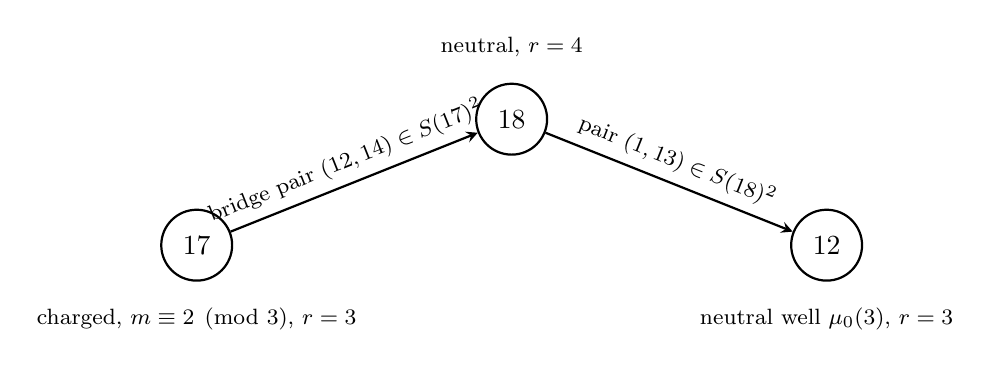
\begin{tikzpicture}[>=stealth, thick,
   vtx/.style={circle,draw,minimum size=9mm,inner sep=1pt}]
\node[vtx] (v17) at (0,0) {$17$};
\node[vtx] (v18) at (4,1.6) {$18$};
\node[vtx] (v12) at (8,0) {$12$};
\draw[->] (v17) -- (v18)
   node[midway,above,sloped]{\footnotesize bridge pair
   $(12,14) \in \rays(17)^{2}$};
\draw[->] (v18) -- (v12)
   node[midway,above,sloped]{\footnotesize pair
   $(1,13) \in \rays(18)^{2}$};
\node[below=2mm of v17]{\footnotesize charged, $m \equiv 2 \pmod 3$,
   $\rch = 3$};
\node[above=2mm of v18]{\footnotesize neutral, $\rch = 4$};
\node[below=2mm of v12]{\footnotesize neutral well $\mu_0(3)$,
   $\rch = 3$};
\end{tikzpicture}
\caption{The order-$2$ escape at level $k = 3$
(Remark~\ref{rem:zigzag}): the charged vertex $17$, confined by
the valve inside its fibre under descending arcs, ascends
through its alive bridge to the neutral vertex $18$
($w = (3m - 3 \pm a)/2 \equiv 0 \pmod 3$), which then descends
to the neutral well $12 = \mu_0(3)$. Richnesses along the path:
$3, 4, 3$.}
\label{fig:zigzag}
\end{figure}

\begin{remark}[diagonal arcs ($a = b$)]\label{rem:diag}
Setting $a = b \in \rays(m)$ in the sum child (with $a < m - 3$ so
that $n \ge 4$ remains in the digraph domain; the extremal ray
$a = m - 3$ would give $n = 3$) yields a unary arc $m \to n = m - a$,
whose child is the lower prime $p = m - a \in [5, m - 1]$ itself.
For a charged $m$ every such non-extremal ray is regular
($a \equiv 0 \pmod 3$), so the diagonal arc stays in the same
charged class ($p \equiv m \pmod 3$), preserves the valve, adds up
to $\rch(m)$ arcs per vertex, and preserves the certificates at
$k \ge 2$; at $k = 1$ it already kills the interior well $19$ (via
$19 \to 7$) and the neutral minimum $6 = \mu_0(1)$ (via $6 \to 5$),
reducing the level-$1$ wells from the $\{4, 5, 6, 7, 19\}$ of the
strict-pair digraph ($a^{\mathrm{win}}(1) = 5$) to $\{4, 5, 7\}$, $7$
remaining the sole interior one.
\end{remark}

\subsection{Dense coverage by \texorpdfstring{$\Delta$}{Delta}-arcs}
\label{sec:dense}

The digraph cannot decide Goldbach at a single vertex
(Remark~\ref{rem:walls}), but it certifies coverage around a
rich one, unconditionally.

\begin{theorem}[local Schnirelmann coverage]\label{thm:dense}
There is an absolute constant $X_0$ such that for every real
$X \ge X_0$, some integer $m \in [X, 2X]$ has descending
$\Delta$-children covering a positive proportion of the integers
below it:
\[
\bigl|C_\Delta^{-}(m)\bigr|
\;\ge\; \max\Bigl\{\, c_1\, m,\;
\frac{c_2\, m}{(\ln\ln m)^{6}} \,\Bigr\}
\]
for absolute constants $c_1, c_2 > 0$ (the first term dominates
asymptotically; the second, explicit in the sieve constants, is
the sharper bound at finite scale). Every child
$n \in C_\Delta^{-}(m) \subset (m/2, m-1]$ carries a prime pair of
$\mathrm{Part}(m)$, hence satisfies $\rch(n) \ge 1$
unconditionally: a single rich vertex generates, in one re-pairing
step, a positive fraction of the even integers $2n$ below $2m$ (a
one-germ analogue of Schnirelmann density~\cite{schnirelmann}).
\end{theorem}

\begin{proof}
Steps 1, 2 and 5 are elementary; Steps 3 and 4 are proved from
the classical Selberg upper sieve for linear forms
(Halberstam--Richert~\cite[Theorem~5.7]{hr}) and an elementary
local-factor comparison; no unproved input remains.

\smallskip
\noindent\emph{Step 1 (rich centre of bounded singular series,
elementary).} Pairs of primes $X < p < q \le 2X$ have integer midpoint
$m = (p + q)/2 \in (X, 2X) \subseteq [X, 2X]$, so Chebyshev's
dyadic bound $\pi(2X) - \pi(X) \ge c'_T X/\ln X$ gives
$\sum_{X < m < 2X} \rch(m) \ge \binom{\pi(2X)-\pi(X)}{2}
\ge c_T\, X^{2}/\ln^{2} X$.
The upper sieve of Step~3 (dimension $\kappa = 2$) also bounds each
$\rch(m) \le K_s\,\mathfrak{S}_2(2m)\,m/\ln^{2} m$;
writing $\mathfrak{S}_2(2m)^{2} = 4C_2^{2}\sum_{d \mid m} h(d)$
on odd squarefree $d$ with
$h(p) = ((p-1)/(p-2))^{2} - 1 = O(2/p)$ gives
$h(p)/p = O(2/p^{2})$, so
$\sum_{m \le Y} \mathfrak{S}_2(2m)^{2} \le K_2 Y$
($K_2 \approx 4.6$). For $X \ge e^{2}$,
$m/\ln^{2} m \le 2X/\ln^{2} X$ on $(X, 2X)$, and Markov's
inequality confines the large-$\mathfrak{S}_2$ mass:
\[
\sum_{\substack{X < m < 2X \\ \mathfrak{S}_2(2m) > \Lambda}}
\rch(m)
\;\le\; \frac{2 K_s\, X}{\ln^{2} X}\cdot \Lambda^{-1}
 \sum_{m \le 2X} \mathfrak{S}_2(2m)^{2}
\;\le\; \frac{4 K_s K_2}{\Lambda}\,
 \frac{X^{2}}{\ln^{2} X} .
\]
Fixing the absolute constant $\Lambda$ with
$8 K_s K_2 / \Lambda < c_T$ leaves at least half of the
Chebyshev mass on vertices whose singular series stays
$\le \Lambda$: some $m \in (X, 2X) \subseteq [X, 2X]$ satisfies
simultaneously
\[
\rch(m) \;\ge\; c_0\, \frac{m}{\ln^{2} m}
\qquad\text{and}\qquad
\mathfrak{S}_2(2m) \;\le\; \Lambda ,
\qquad c_0, \Lambda > 0 \ \text{absolute}.
\]
The bound $\mathfrak{S}_2(2m) \le \Lambda$ is essential:
$\mathfrak{S}_2(2m) \asymp m/\varphi(m)$ is unbounded on
primorials, so no choice of centre skipping it would leave an
absolute constant below.

\smallskip
\noindent\emph{Step 2 (combinatorial identity).}
Each unordered pair $a < b$ of rays produces the $\Delta$-child
$n = m - (b-a)/2$; let $w_\Delta(m,n)$ count the pairs generating
$n$, so $\binom{\rch(m)}{2} = \sum_n w_\Delta(m,n)$ and
Cauchy--Schwarz on the support gives
\begin{equation}\label{eq:D1}\tag{D1}
\bigl|C_\Delta^{-}(m)\bigr|
 \;\ge\; \frac{\binom{\rch(m)}{2}^{2}}
 {\displaystyle\sum_{n < m} w_\Delta(m,n)^{2}} .
\end{equation}

\smallskip
\noindent\emph{Step 3 (upper sieve, unconditional).}
For fixed $d = m - n$ with $1 \le d < m/2$ (a $\Delta$-arc only
reaches the upper half $n > m/2$, Remark~\ref{rem:dsarc}, which
keeps the resultant below nonzero), $w_\Delta(m,n)$ counts
$a \in [1, m]$ with all four linear forms
$L_i(a) \in \{m - a,\ m + a,\ m - a - 2d,\ m + a + 2d\}$ prime;
counting $|L_i(a)| \in \mathbb{P}$ over the whole interval
majorises this and removes any degeneracy of $\ln(m - 2d)$ as
$d \to m/2$. Define the associated degree-$4$ singular series
\[
\mathfrak{S}_4^{\Delta}(m, d)
 \;=\; \prod_{\ell \ge 2} \mathrm{loc}_4^{\Delta}(\ell; m, d),
\qquad
\mathrm{loc}_4^{\Delta}(\ell; m, d)
 \;=\; \frac{\ell^{3}(\ell - \nu_\ell(m,d))}{(\ell - 1)^{4}},
\]
where $\nu_\ell(m,d) = |\{m, -m, m - 2d, -m - 2d\} \bmod \ell|$
counts the distinct roots of $\prod_{i=1}^4 L_i(a) \equiv 0
\pmod \ell$ (note that $\nu_2(m,d) = 1$ always, whereas unlike
$\mathfrak{S}_4^{\mathrm{bn}}$ in Definition~\ref{def:bottleneck},
$3 \nmid d$ is permitted here so $\nu_3(m,d) = 3$ can occur, in
which case $\mathfrak{S}_4^{\Delta}(m,d) = 0$). The Selberg upper
sieve of dimension $\kappa = 4$ for linear forms in one variable,
applied at level $\xi = m^{1/2}(\ln m)^{-B}$ ($B \ge 4$,
\cite[Theorem~5.7]{hr}), bounds the quadruple count by
\begin{equation}\label{eq:HA}\tag{$H_A$}
w_\Delta(m,n) \;\le\; (384 + O(\ln\ln m/\ln m))\,
\mathfrak{S}_4^{\Delta}(m, d)\, \frac{m}{\ln^{4} m}
\;+\; O\bigl(m\,(\ln m)^{3-2B}\bigr) ,
\end{equation}
uniformly in $d$: the additive term is the sieve remainder
$\sum_{[d_1,d_2] < \xi^{2}} 4^{\omega([d_1,d_2])}
\ll \xi^{2}(\ln \xi)^{3} = m(\ln m)^{3-2B}$ (dominating the
$\le 8\xi$ values of $a$ where some $|L_i(a)| \le \xi$), while
the system resultant
$|E| = 64\, m^{2} d^{2} (m^{2} - d^{2}) \ne 0$ satisfies
$\ln\ln(3|E|) \le \ln\ln m + O(1)$, so the error term
$O(\ln\ln m / \ln m)$ of \cite[Theorem~5.7]{hr} is automatic.
The constant is $2^{4} \cdot 4! = 384$: the simplex volume
$1/\kappa!$ of the degree-$4$ upper sieve, not the naive
parity loss $2^{4} = 16$. Two cases are distinguished. If
$\nu_p(m,d) = p$ for some prime $p$ (which can only occur at
$p = 3$, when $3 \nmid m$ and $3 \nmid d$, as
$\{m, -m, m - 2d, -m - 2d\}$ then exhausts $\mathbb{Z}/3\mathbb{Z}$
while $\nu_2 = 1$ always), every $a$ makes some $|L_i(a)|$ a
multiple of $3$, hence $|L_i(a)| = 3$: at most $8$ values of $a$ in
all, so $w_\Delta(m,n) \le 8$ elementarily, absorbed into the
additive term of~\eqref{eq:HA}. Otherwise $\nu_p(m,d) < p$ for
every $p$, $\mathfrak{S}_4^{\Delta}(m,d) > 0$, and
\cite[Theorem~5.7]{hr} applies literally.

\smallskip
\noindent\emph{Step 4 (second moment and sup bound, unconditional).}
Comparing the local factors $\mathrm{loc}_4^{\Delta}(p;m,d)$ with
$\mathrm{loc}_2(p;m)^{2}$, the combined ratio across $p \in \{2,3\}$
is at most $2 \cdot 3 = 6$ (namely $8/4 = 2$ at $p = 2$ and at most
$27/9 = 3$ at $p = 3$); for $p \ge 5$ it is $\le 1$ unless
$p \mid d(m - d)(m + d)$, in which case it is $\le p/(p-2)$. Hence
pointwise
$\mathfrak{S}_4^{\Delta}(m, d) \le 6\,\mathfrak{S}_2(2m)^{2}\,
f(d)\, f(m-d)\, f(m+d)$ with
$f(k) = \prod_{p \mid k,\, p \ge 5} p/(p-2)$. Since
$f(k)^{6} = \sum_{r \mid k} g(r)$ with
$g(p) = (p/(p-2))^{6} - 1 \sim 12/p$ ($g \ge 0$ on squarefree
$r$), the triple H\"older inequality bounds
$\sum_{1 \le d < m/2} (f(d)f(m-d)f(m+d))^{2}$ by the geometric mean
of the three disjoint partial sums $\sum_{d < m/2} f(d)^{6}$,
$\sum_{d < m/2} f(m-d)^{6}$ and $\sum_{d < m/2} f(m+d)^{6}$, hence
\emph{a fortiori} by one third of the total over $k < 3m/2$
(arithmetic--geometric mean), giving the prefactor $6^{2}/3 = 12$
of \eqref{eq:HB}; and
$\sum_{k \le Y} f(k)^{6} = \sum_{r \le Y} g(r)\lfloor Y/r\rfloor
\le Y\sum_{r \ge 1} g(r)/r$:
\begin{equation}\label{eq:HB}\tag{$H_B$}
\sum_{1 \le d < m/2} \mathfrak{S}_4^{\Delta}(m, d)^{2}
 \;\le\; 12\,\mathfrak{S}_2(2m)^{4}
 \sum_{k < 3m/2} f(k)^{6}
 \;\le\; 18\, C_6\, m\,\mathfrak{S}_2(2m)^{4},
\qquad C_6 = \prod_{p \ge 5}\Bigl(1 + \frac{g(p)}{p}\Bigr)
 \approx 17.5 .
\end{equation}
The same local-factor comparison also gives a uniform supremum
bound: $f(k) \ll (\ln\ln k)^{2}$ (the product over distinct primes
is maximised on initial segments, so
$\ln f(k) \le \sum_{5 \le p \le y} 2/(p-2) + O(1)
= 2\ln\ln y + O(1)$ with $y \sim \ln k$ by Mertens' theorem), hence
uniformly in $1 \le d < m/2$,
\begin{equation}\label{eq:HC}\tag{$H_C$}
\mathfrak{S}_4^{\Delta}(m,d)
 \;\le\; C_s\,\mathfrak{S}_2(2m)^{2}\,(\ln\ln m)^{6},
\end{equation}
with $C_s > 0$ absolute.

\smallskip
\noindent\emph{Step 5 (assembly).} Inserting \eqref{eq:HA} and
\eqref{eq:HB} into \eqref{eq:D1} at the centre $m$ of Step~1
($\mathfrak{S}_2(2m) \le \Lambda$; also $w_\Delta(m,n) = 0$ for
$d = m - n \ge m/2$, so the sum ranges over $1 \le d < m/2$ as in
\eqref{eq:HB}) yields
\[
\sum_{n < m} w_\Delta(m,n)^{2}
 \;\le\; (384 + o(1))^{2}\cdot 18\, C_6\, \Lambda^{4}\,
 \frac{m^{3}}{\ln^{8} m} ,
\]
the additive $O(m(\ln m)^{3-2B})$ of \eqref{eq:HA} (which is
$O(m/\ln^{5} m)$ for $B \ge 4$) contributing through the
cross-term $O(m^{3}/\ln^{9} m) = o(m^{3}/\ln^{8} m)$ only; thus
\[
\bigl|C_\Delta^{-}(m)\bigr| \;\ge\;
\frac{\binom{\rch(m)}{2}^{2}\,\ln^{8} m}
 {(384 + o(1))^{2}\, 18\, C_6\, \Lambda^{4}\, m^{3}} ,
\]
and, taking $X_0$ large enough so that
$\rch(m) \ge c_0 m/\ln^{2} m \ge 2$, the bound
$\binom{\rch(m)}{2} \ge \rch(m)^{2}/4 \ge
c_0^{2} m^{2}/(4\ln^{4} m)$ gives
$\bigl|C_\Delta^{-}(m)\bigr| \ge c_1\, m$ with
\[
c_1 \;=\; \frac{c_0^{4}}
 {7.5 \times 10^{8}\, \Lambda^{4}} \;>\; 0
\quad\text{absolute}
\]
($16 \times 384^{2} \times 18\, C_6 \approx 7.44 \times 10^{8} <
7.5 \times 10^{8}$, absorbing the $o(1)$ for $X \ge X_0$; the
$\mathfrak{S}_2(2m)^{4}$ of \eqref{eq:HB} is replaced by
$\Lambda^{4}$, a pure number, thanks to the
bounded-singular-series choice of $m$). A second, sup-norm
assembly avoids squaring the sieve constant altogether: by the
fibre identity, $\sum_{n<m} w_\Delta(m,n)^{2} \le
(\max_{n<m} w_\Delta(m,n))\cdot\binom{\rch(m)}{2}$, and combining
\eqref{eq:HA} with \eqref{eq:HC} gives
$\max_{n<m} w_\Delta(m,n) \le
(384 + o(1))\,C_s\,\Lambda^{2}(\ln\ln m)^{6}\,m/\ln^{4}m$
(the additive error $O(m\ln^{-5}m)$ of \eqref{eq:HA} being absorbed
again); hence, absorbing the $o(1)$ for $X \ge X_0$ into the margin
$384 \to 385$,
\[
\bigl|C_\Delta^{-}(m)\bigr|
\;\ge\; \frac{\binom{\rch(m)}{2}}{\max_{n<m} w_\Delta(m,n)}
\;\ge\; \frac{c_0^{2}}{4\cdot 385\, C_s\,\Lambda^{2}}\,
\frac{m}{(\ln\ln m)^{6}}
\;=\; \frac{c_2\,m}{(\ln\ln m)^{6}} ,
\]
completing the proof of both bounds.
\end{proof}

\begin{remark}[effectivity, heuristic size, and optimality of the sieve factor]
\label{rem:densesize}
In the second bound of Theorem~\ref{thm:dense}, $384$ enters only
to the \emph{first} power and $\mathfrak{S}_2(2m)$ only as
$\Lambda^{2}$, at the price of $(\ln\ln m)^{6}$: it dominates
$c_1 m$ below a double-exponential threshold, and remains
non-trivial whenever $\rch(m) \ge c_0 m/\ln^{2} m$. Note further
that the proof uses only the Selberg sieve on $\mathbb{Z}$ and
Chebyshev's bound (no Dirichlet characters and no
Bombieri--Vinogradov theorem~\cite{bombieri,vinogradovA}), so $c_1$,
$c_2$, and $X_0$ are \emph{effective in principle} (free of
Siegel-zero ineffectivity). Heuristically, replacing the H\"older
majorant in~\eqref{eq:HB} by the expected local second moment
$\sum_{d<m/2} \mathfrak{S}_4^{\Delta}(m,d)^{2} \sim
(\kappa_4(m)/2)\, m\,\mathfrak{S}_2(2m)^{4}$ would raise $c_1$ to
the order of $c_0^{4}\Lambda^{-4}/(8\kappa_4(m)\cdot 384^{2}) \approx
10^{-7}\, c_0^{4}\Lambda^{-4}$, where
$\kappa_4(m) = 4\, M_2(3;m) \prod_{p \ge 5} M_2(p;m)$ with
$M_2(3;m) = 9/8$ or $3$ according to $3 \mid m$ or $3 \nmid m$, and
$M_2(p;m) = 1 + (p-1)^{-3}$ ($p \mid m$) or
$1 + (6p-16)/(p-2)^{4}$ ($p \nmid m$), so $\kappa_4(m) \approx
5$--$15$ ($\kappa_4(m) \ge 4$ by Cauchy--Schwarz, as $p=2$
contributes a constant ratio $2$). Finally, the degree-$4$ sieve
factor $2^{4} \cdot 4! = 384$ is optimal for the method: although
the root set $\{m,-m,m-2d,-m-2d\}$ is the tensor product
$\{\pm m\}\otimes\{0,-2d\}$, restricting the $\Lambda^{2}$ weights
to products $\rho_1(d_1)\rho_2(d_2)$ only shrinks the feasible set
of the sieve's quadratic form (the four forms share one variable),
so no tensor-power decomposition beats $2^\kappa \kappa!$ below the
parity barrier.
\end{remark}

\begin{remark}[kernel verification]\label{rem:leandense}
The combinatorial part of Theorem~\ref{thm:dense} is
machine-verified by the Lean artefact (Appendix~\ref{app:lean},
zero \texttt{sorry}): strict descent of $\Delta$-children, the
fibre identity and the pair count by swap symmetry, support
Cauchy--Schwarz~\eqref{eq:D1}, and the final assembly. In the
artefact the sieve bounds \eqref{eq:HA} and \eqref{eq:HB} appear as
explicit parameters, never as axioms; the proof above discharges
them through \cite[Theorem~5.7]{hr} and the elementary local-factor
estimate, so the theorem as stated is unconditional. The additional
input~\eqref{eq:HC} is discharged by the same local-factor estimate
and is used only in the paper-side sup-norm assembly. What the
kernel certifies is therefore exactly the non-analytic skeleton of
the theorem.
\end{remark}

\subsection{Measured windows}

\begin{table}[htbp]
\centering
\caption{Complete list of the two-well windows ($a^{\mathrm{win}}(k)=2$)
measured on the richness-table zone: $52$ windows for
$3 \le k \le 14\,089$ (single-level windows are written as
singletons $\{k\}$); the last certified two-well threshold is
$k = 14\,089$.}
\label{tab:windows}
\begin{tabular}{@{}llll@{}}
\toprule
$[3,13]$ & $[15,20]$ & $[27,28]$ & $[30,33]$\\
$[35,41]$ & $[47,48]$ & $[52,58]$ & $[79,82]$\\
$[86,90]$ & $[93,101]$ & $\{103\}$ & $[115,117]$\\
$[153,158]$ & $[171,172]$ & $[208,231]$ & $\{238\}$\\
$[354,385]$ & $[415,426]$ & $[480,482]$ & $[485,492]$\\
$[526,528]$ & $[547,549]$ & $[584,604]$ & $[634,649]$\\
$[656,676]$ & $[759,781]$ & $[920,944]$ & $[1\,097,1\,144]$\\
$[1\,277,1\,291]$ & $[1\,308,1\,355]$ & $[1\,426,1\,427]$ & $\{1\,688\}$\\
$[1\,835,1\,838]$ & $[2\,096,2\,108]$ & $[2\,183,2\,186]$ & $[2\,264,2\,278]$\\
$[2\,616,2\,631]$ & $[2\,646,2\,693]$ & $[3\,046,3\,055]$ & $[3\,350,3\,501]$\\
$[3\,713,3\,855]$ & $[3\,974,4\,047]$ & $[4\,477,4\,503]$ & $[4\,552,4\,708]$\\
$[6\,747,6\,816]$ & $[8\,103,8\,242]$ & $[8\,465,8\,492]$ & $[9\,673,9\,745]$\\
$[9\,832,9\,996]$ & $[10\,166,10\,234]$ & $[10\,436,10\,609]$ & $[14\,021,14\,089]$\\
\bottomrule
\end{tabular}
\end{table}

The thresholds $k = 512$ and $k = 1\,024$ of Table~\ref{tab:chk1m}
happened to fall inside three-well zones
($a^{\mathrm{win}}(512) = a^{\mathrm{win}}(1\,024) = 3$).

\begin{remark}[the last window is open-ended]\label{rem:lastwin}
The final window $k \in [14\,021, 14\,089]$ is generated by
$\mu_{\max} = 994\,175$ (class $2$): its bridge is alive
($2\mu_{\max} - 3 = 1\,988\,347$ is prime) and emits $28\,176$
bridge-children, of maximal richness $r = 14\,324$. The window
presumably runs on to $k = 14\,324$, but $\mu_2(k)$ for
$k > 14\,089$ lies outside the richness table: only
$[14\,021, 14\,089]$ is certified.
\end{remark}

\begin{remark}[why no permanent regime is conjectured (heuristic)]
\label{rem:hl3}
Under a Hardy--Littlewood-type model for prime triples, the bridge
$2\mu_{\max}-3$ never dies permanently: the probability that
$2\mu_{\max}-3$ is prime behaves like
$\ln\ln \mu_{\max} / \ln \mu_{\max}$, amplified on primorials by
the singular series. Relapses $3 \to 2$ are therefore expected at
every horizon: the well count should have \emph{no limit}, and the
stable form ``$a(k) \ge 3$ for all $k \ge k_c$'' is \emph{not}
conjectured. This paragraph is a heuristic model, not a theorem.
\end{remark}

\section{Conjectures and models}
\label{sec:conj}

\subsection{The three main conjectures}

We begin by formulating the three main conjectures announced in the
abstract: the master margin conjecture governing the absence of
interior wells (and hence the global well count), the charged
bottleneck conjecture for prime quadruples at gaps divisible by $6$,
and the perpetual oscillation conjecture with asymptotic density one
at three wells.

\begin{conjecture}[\textsc{conj-m}: master margin conjecture]
\label{conj:M}
For every integer $m \ge 4$ with $\tau(m) \ge 2$,
\[
\delta(m) \;=\; M(m) - \tau(m) \;\ge\; 0 .
\]
Equivalently, no vertex of $\Dk$ ($k \ge 2$) is an interior well.
\end{conjecture}

\begin{remark}[record level $1$ and empirical status of \textsc{conj-m}]
Conjecture~\ref{conj:M} is open; in Section~\ref{sec:data} we
measured $0$ interior wells among $999\,947$ vital vertices with
$\tau(m) \ge 2$ on $[6, 999\,958]$, and $0$ among the $290\,177$
vital vertices with $\tau(m) \ge 7\,227$ on $[6, 10^{6}]$. On the window,
the landscape is sharper at record level $1$: the only vertices
with $\tau(m) \ge 1$ and $\delta(m) < 0$ are $m \in \{7, 19\}$, the
two non-minimum wells of $D_1$. That level-$1$ clause is logically
independent of Conjecture~\ref{conj:M} (a putative $m > 19$ with
$\rch(m) = 1$ would have $\tau(m) = 1$ and $\delta(m) < 0$ while
satisfying Conjecture~\ref{conj:M} vacuously), and has
tail-hypothesis content (asserting in particular that no $m > 19$
has $\rch(m) = 1$).
\end{remark}

\begin{conjecture}[\textsc{conj-a}: shifted Dubner-type bottleneck conjecture]
\label{conj:A}
For every charged dead-bridge bottleneck pair $(u_1,u_2,k,c)$
($c \in \{1,2\}$, $2u_2 - 3$ composite),
\[
N(u_1,u_2) \;=\; r_{\mathrm{Part}(u_2)}(u_1) \;\ge\; 1.
\]
Equivalently (by Theorem~\ref{thm:bij}), $u_1 \in C^{-}(u_2)$: at
every charged dead-bridge bottleneck, the prime quadruple
$(p,\ p+2v,\ 2u_1-p,\ 2u_2-p)$ ($v = u_2 - u_1$) admits at least
one witness $p \in [3, u_1 - 1] \setminus \{2u_1 - u_2\}$.
\end{conjecture}

\begin{conjecture}[\textsc{conj-osc}: perpetual oscillation, density one at three wells]
\label{conj:OSC}
For every integer $k \ge 3$, $a(k) = |\wells(\Dk)| \in \{2,3\}$, with
\[
\liminf_{k \to \infty} a(k) = 2, \qquad
\limsup_{k \to \infty} a(k) = 3, \qquad
\lim_{K \to \infty} \frac{|\{3 \le k \le K : a(k) = 3\}|}{K} = 1 .
\]
Equivalently, $a(k) = 2 + (1 - \beta(k))$ for a binary sequence
$\beta(k) \in \{0,1\}$ encoding the retention of a bridge arc from
$\mu_{\max}(k)$.
\end{conjecture}

\begin{remark}[mechanism and measured decay]\label{rem:oscdecay}
Conjecture~\ref{conj:OSC} is open. Taking the contrapositive
of Theorem~\ref{thm:cert3} via Theorem~\ref{thm:bridge}: under the regime
$\mu_0(k) < \min(\mu_1(k),\mu_2(k))$, the event $a(k) = 2$ forces
$2\mu_{\max}(k) - 3$ to be prime. Even on primorial champions,
Mertens' bound caps that primality probability heuristically at
$\sim e^\gamma \ln\ln \mu_{\max} / \ln(2\mu_{\max})
\asymp \ln\ln K / \ln K \to 0$, while the sum over champions
diverges and preserves $\liminf_{k\to\infty} a(k) = 2$. On the
measured window, the two-well share already decays
(Table~\ref{tab:windows}): $56/98$ ($57.1\,\%$) on $k \in [3,100]$,
$205/900$ ($22.8\,\%$) on $[101,1\,000]$, $777/4\,000$ ($19.4\,\%$)
on $[1\,001,5\,000]$, and $788/9\,089$ ($8.7\,\%$) on
$[5\,001,14\,089]$.
\end{remark}

\subsection{Auxiliary ceiling conjectures and logical implications}

We next record the global three-well ceiling, prove its unconditional
deduction (together with Conjecture~\ref{conj:A}) from
Conjecture~\ref{conj:M} in ZFC, and state two refined ceiling
variants on restricted arc sub-digraphs.

\begin{conjecture}[\textsc{conj-b}: three-well ceiling]
\label{conj:B}
For every integer $k \ge 2$, $a(k) = |\wells(\Dk)| \le 3$.
\end{conjecture}

\begin{proposition}[unconditional consequences of \textsc{conj-m}]
\label{prop:master}
In ZFC (without assuming the tail hypothesis $H(k)$),
Conjecture~\ref{conj:M} implies both Conjecture~\ref{conj:B} and
Conjecture~\ref{conj:A}.
\end{proposition}

\begin{proof}
Assume Conjecture~\ref{conj:M}. Fix $k \ge 2$. Each fibre
$\Vk \cap \{m \equiv c \pmod 3\}$, $c \in \{0,1,2\}$, is nonempty
(Lemma~\ref{lem:fibres}) and has a unique minimum $\mu_c(k)$ by
well-ordering, even if $L_k = +\infty$. Every non-minimum vertex
$m \in \Vk$ in class $c$ satisfies $\mu_c(k) < m$ with
$\rch(\mu_c(k)) \ge k$ and $\rch(m) \ge k$, so
$\tau(m) = \min(\rch(m), R(m)) \ge k \ge 2$. By
Conjecture~\ref{conj:M}, $M(m) \ge \tau(m) \ge k$, meaning that $m$
emits a retained descending arc in $\Dk$ and is not a $k$-well.
Hence $\wells(\Dk) \subseteq \{\mu_0(k),\mu_1(k),\mu_2(k)\}$, which
yields $a(k) \le 3$, proving Conjecture~\ref{conj:B}.

Next, let $(u_1,u_2,k,c)$ be a charged dead-bridge bottleneck pair
($c \in \{1,2\}$, $2u_2 - 3$ composite). We first verify $k \ge 3$
unconditionally: in class~$1$, $\rch(7) = 1$, $\rch(10) =
\rch(13) = 2$, and the initial challengers $(7,10)$ and $(10,13)$
have alive bridges ($17$ and $23$ are prime); in class~$2$,
$\rch(8) = \rch(11) = 2$ and $(8,11)$ has an alive bridge ($19$ is
prime). Every subsequent challenger in class $1$ or $2$ must
strictly exceed the second-largest richness $\ge 2$, forcing
$k \ge 3$. Since $\rch(4) = \rch(5) = 1 < k$, Definitions~\ref{def:bottleneck}
and~\ref{def:margin} give $R(u_2) = \rch(u_1)$ and
$\tau(u_2) = \min(\rch(u_2),\rch(u_1)) = k \ge 3$. By
Conjecture~\ref{conj:M}, $M(u_2) \ge k$, so there exists
$n \in C^{-}(u_2)$ with $\rch(n) \ge k$. Corollary~\ref{cor:dead}
confines $n < u_2$ to class $c$ modulo~$3$, and $\rch(n) \ge 3$
forces $n \ge 6$. The strict bottleneck inequality
$k > \max\{\rch(w) : 6 \le w < u_2,\ w \neq u_1,\ w \equiv c \pmod 3\}$
leaves $n = u_1$ as the unique candidate, so $u_1 \in C^{-}(u_2)$,
and Theorem~\ref{thm:bij} yields $N(u_1,u_2) \ge 1$, proving
Conjecture~\ref{conj:A}.
\end{proof}

\begin{remark}[fineness of \textsc{conj-m} and scope of \textsc{conj-a}]
\label{rem:posA}
Conjecture~\ref{conj:M} is strictly finer than
Conjecture~\ref{conj:B}: a single interior well inside a two-well
window would still yield $2 + 1 = 3$ wells and satisfy
Conjecture~\ref{conj:B}, whereas Conjecture~\ref{conj:M} forbids it.
Likewise, for non-bottleneck vital vertices, or if the strict inequality in
Definition~\ref{def:bottleneck} is relaxed to allow ties, the
margin inequality only forces \emph{some} earlier class-record
vertex to lie in $C^{-}(u_2)$, whereas the rank-$2$ leader pass
tests drainage to the immediate leader; Conjecture~\ref{conj:A} is
stated separately among the main conjectures for its explicit
prime-quadruple content.
\end{remark}

\begin{remark}[honest position on the ceiling]
Conjecture~\ref{conj:B} needs no $H(k)$ once Conjecture~\ref{conj:M}
is granted; independently, under $H(k)$ alone,
Proposition~\ref{prop:mcut} confines every well to
$[4, \Mcut(k,L_k) - 1]$ and decides each $k$ on that finite range.
Even under $H(k)$, however, the bound $a(k) \le 3$ requires that
\emph{every} candidate beyond the class minima be covered: the
absence of interior wells is \emph{not} deduced from the
certificates: it is the measured point ($0$ interior wells in the
window).
\end{remark}

\begin{conjecture}[\textsc{conj-b}$\Delta$: the $\Delta$-only ceiling]
\label{conj:Bdelta}
Let $a_\Delta(k) = |\wells(\DkD)|$ be the well count of the
difference-arc sub-digraph on $\Vk$. Then $a_\Delta(k) \in \{2,3\}$
for every integer $k \ge 3$.
\end{conjecture}

Conjecture~\ref{conj:Bdelta} is open and strictly stronger than
Conjecture~\ref{conj:B}: removing $\Sigma$-arcs removes escapes, so
$a_\Delta(k) \ge a(k)$, and any counterexample $a_\Delta(k) \ge 4$
in $[4,10^6]$ is directly testable on the richness table.

\begin{remark}[where $\Delta$-only wells could hide]
\label{rem:deltagap}
The inclusion $\wells(\Dk) \subseteq \wells(\DkD)$ gives
$a_\Delta(k) \ge a(k)$ for every $k$; a strict gap
$a_\Delta(k) > a(k)$ corresponds to a vertex with all
$\Delta$-children below level $k$ but some $\Sigma$-child at level
$\ge k$. Proposition~\ref{prop:sigmabridge} does \emph{not} imply
equality: it only rules out retained bridge $\Sigma$-arcs at
$\mu_{\max}(k)$, while (i) any $\Sigma$-arc factorisable through a
two-step $\Delta$-path loses its relay if the relay drops below $k$
(threshold effect), and (ii) in the intra-class band
$\mu_c(k) < m < 2 \mu_c(k)$ a non-monotone $\rch$ can put a smaller
$n_\Sigma$ on a primorial-rich residue ($\mathfrak{S}_2$ large,
$\rch \ge k$) while all $\binom{k}{2}$ children $n_\Delta$ fail.
Heuristically, the probability of such a simultaneous failure decays
like $\exp(-c k^{2})$: gaps, if they exist, concentrate at small $k$
on intra-class vertices just above $\mu_c(k)$.
\end{remark}

\begin{conjecture}[\textsc{conj-2thick}: eventual stabilisation on $2$-thick arcs]
\label{conj:2thick}
For each $k \ge 1$, let $\Dk^{(2)}$ be the sub-digraph on $\Vk$
retaining only $2$-thick descending arcs ($m \to n$ with $n < m$,
$\rch(n) \ge k$, and multiplicity $w(m,n) \ge 2$). There exists an
integer $k_2 \ge 3$ such that for all $k \ge k_2$,
\[
\bigl|\wells\bigl(\Dk^{(2)}\bigr)\bigr| \;=\; 3 .
\]
\end{conjecture}

\begin{remark}[motivation for \textsc{conj-2thick}]
Conjecture~\ref{conj:2thick} is open. By Proposition~\ref{prop:thick},
every charged crossing arc has multiplicity $w(m,n) \le 1$, so the
$2m - 3$ bridge is algebraically switched off in $\Dk^{(2)}$ at
every level: both charged fibres are downward-closed, and whenever
$\mu_0(k) < \min(\mu_1(k),\mu_2(k))$, all three class minima belong
to $\wells(\Dk^{(2)})$ unconditionally in ZFC (with no primality
condition on $2\mu_{\max}(k) - 3$). Heuristically, since the
intra-class witness expectation $\lam$ diverges and the Poisson tail
$(1 + \lam)\exp(-\lam)$ is summable over bottlenecks, $2$-thick
intra-class drainage should eventually eliminate all interior wells
above some threshold $k_2$: the $\{2,3\}$ windows of $\Dk$ are
precisely the multiplicity-$1$ bridge escapes.
\end{remark}

\subsection{Quantitative structure of the bottleneck conjecture}

Conjecture~\ref{conj:A} is a Dubner-type statement~\cite{dubner,oeis}
on prime pairs at a forced gap, shifted to the admissible case
$6 \mid 2v$: the two vertices of a bottleneck share a class
$c \in \{1,2\}$ modulo~$3$, so $v = u_2 - u_1 \equiv 0 \pmod 3$.

\begin{remark}[admissibility is forced]
The condition $6 \mid 2v$ is not a choice: for $p > 3$ and
$2v \not\equiv 0 \pmod 6$ the quadruple hits a mod-3 obstruction: one
of $p$, $p+2v$, $2u_1 - p$, $2u_2 - p$ is a multiple of $3$ larger
than $3$. The bottleneck lives exactly in the admissible case.
Conjecture~\ref{conj:A} is open; on the window $[4,10^6]$, it holds
for $358/358$ charged dead-bridge bottlenecks ($674/674$ including
the $316$ neutral pairs), with median $N/\lam \approx 0.99$.
\end{remark}

\begin{remark}[quantitative form]\label{rem:quantA}
The measured amplification suggests the stronger statements
$N(u_1,u_2) \to +\infty$ along bottlenecks ($k \to \infty$) and
the leader law $\kappa(u_1,u_2) \asymp (\ln\ln k)^2$: every prime
$\ell \ge 5$ dividing $\gcd(u_1,u_2)$ gives $\nu_\ell = 1$ in
$\mathfrak{S}_4^{\mathrm{bn}}$ and multiplies
$\kappa = \mathfrak{S}_4^{\mathrm{bn}}(u_1,u_2)/\mathfrak{S}_2(2u_1)$
by $(\ell-2)/(\ell-4)$. On leaders divisible by the primes
$5 \le \ell \le y$ with $y \asymp \ln k$ the product telescopes
and diverges like $(\ln\ln k)^2$; already
$5 \cdot 7 \cdot 11 \cdot 13 \cdot 17 \mid \gcd(u_1,u_2)$ yields
$\kappa \ge \dfrac{C_4}{2C_2}\cdot\dfrac{825}{91}
= 3.144 \times 9.066 \approx 28.5$, which accounts for the
measured $\kappa_{\mathrm{eff}} \sim 30$ of
Section~\ref{sec:bottlenecks} with no free parameter and predicts
$N(u_1,u_2) \asymp k (\ln\ln k)^2 / \ln^2 k$ on primorial leaders.
\end{remark}

\begin{remark}[arity-$2$ normalisation: $C_4$ and $C_2$ cancel]
\label{rem:lambda2}
The midpoint reading suggests the self-normalised predictor
\[
\Lambda_2(u_1,u_2)
 \;=\; \rch(u_1)\Bigl(\frac{\rch(u_2)\,\ln(2u_2)}{u_2}\Bigr)^2
 \;=\; \frac{\rch(u_1)\,\rch(u_2)^2\,(\ln(2u_2))^2}{u_2^2},
\]
built from the observed densities of the partner sets rather than
from singular-series constants. Writing
$\mathfrak{S}_4^{\mathrm{bn}}(u_1,u_2) =
\prod_{\ell \ge 2}\mathrm{loc}_4^{\mathrm{bn}}(\ell)$ and
$\mathfrak{S}_2(2m) = \prod_{\ell \ge 2}\mathrm{loc}_2(\ell;m)$ as
full Euler products
($\mathrm{loc}_4^{\mathrm{bn}}(\ell) =
\ell^{3}(\ell-\nu_{\ell})/(\ell-1)^{4}$, with
$\mathrm{loc}_2(2;m) = 2$ and $\mathrm{loc}_2(3;m) = 3/2$ if
$3 \mid m$, $3/4$ otherwise), every prime $\ell \ge 5$ dividing
$u_2$ contributes ratio
$\mathrm{loc}_4^{\mathrm{bn}}(\ell)/
 \bigl(\mathrm{loc}_2(\ell;u_1)\,\mathrm{loc}_2(\ell;u_2)^{2}\bigr)
 = 1$ identically (whether $\ell \mid u_1$ or not: the oscillatory
factor $(\ell-2)^{3}/\bigl((\ell-4)(\ell-1)^{2}\bigr)$ cancels the
$\ell$-factor of $C_4/(2C_2)^{3}$ prime-by-prime), generic primes
$\ell \nmid u_2(u_2-u_1)(2u_2-u_1)$ (and $\ell \mid u_1$,
$\ell \nmid u_2$) contribute $1 - O(\ell^{-2})$, while primes
$\ell \nmid u_2$ dividing $(u_2-u_1)(2u_2-u_1)$ contribute
$1 + O(\ell^{-1})$; at $2$ and $3$ the ratio is
$1 \cdot 2^{2} = 2^{2}$ on charged fibres and
$1 \cdot 1 = 1$ on neutral ones. The bottleneck conjecture then
quantifies heuristically as
\[
\frac{r_{\mathrm{Part}(u_2)}(u_1)\cdot u_2^{2}}
     {\rch(u_1)\,\rch(u_2)^2\,(\ln(2u_2))^2}
 \;\longrightarrow\;
 \begin{cases} 2^2 & \text{charged fibre},\\ 1 & \text{neutral fibre},
 \end{cases}
\]
along primorial-type bottlenecks whose smallest prime
non-divisor of $u_2$ satisfies $\ell_0(u_2) \gg \ln u_2$
(and $u_1/u_2 \to 1$). Measured on the $674$ dead-bridge records:
mean $3.10$ (median $3.15$) charged, mean $0.78$ (median $0.78$)
neutral: the $4/1$ split is already visible at $10^{6}$.
\end{remark}

\begin{remark}[$N = N_\Delta + N_\Sigma$ on a bottleneck]
\label{rem:Nsplit}
The witness window $[3, u_1 - 1]$ splits at
$2u_1 - u_2 = u_1 - v$: partners $p < 2u_1 - u_2$ force
$q = 2u_1 - p > u_2$ and generate a $\Delta$-witness (window
length $u_1 - v - 3$ when $u_2 \le 2u_1 - 3$), while
$p > 2u_1 - u_2$ gives a $\Sigma$-witness (length
$\min(v - 1,\, u_1 - 3)$). Hence
\[
N(u_1,u_2) \;=\; N_\Delta(u_1,u_2) + N_\Sigma(u_1,u_2),
\qquad
N_\Delta(u_1,u_2) = 0 \ \ \text{if}\ \ u_2 \ge 2u_1 - 3 :
\]
on large initial jumps only $\Sigma$-arcs carry the descent,
whereas $u_2/u_1 \to 1$ concentrates the mass on
$N_\Delta / N \approx 2 - u_2/u_1 \to 1$.
\end{remark}

\begin{remark}[Poincar\'e series and the $E_2$ predictor]
\label{rem:poincare}
The binary integral $I_2(m) = \int_3^{m-1} \frac{\dd p}{\ln p\,
\ln(2m-p)}$ develops asymptotically in powers of $1/L$,
$L = \ln(2m)$, the symmetry $w \leftrightarrow 1 - w$ cancelling
every $\ln 2$ term; the order-$2$ truncation reads
\[
I_2(m) \;=\; \frac{m}{L^2}\Bigl(1 + \frac{2}{L}
 + \frac{6 - \pi^2/6}{L^2} + O\Bigl(\frac{1}{L^3}\Bigr)\Bigr),
\]
reducing the quadrature error at $m = 10^{5}$ from $\sim 19\,\%$ to
$\sim 1\,\%$ (order $3$ would introduce $\zeta(3)$). This gives the
observable predictor
\[
E_2(u_1,u_2) \;=\;
2^{\,2 \cdot \mathbf{1}_{\{3 \nmid u_2\}}}\;
\rch(u_1)\Bigl(\frac{2\,\rch(u_2)}{\pi(2u_2)}\Bigr)^{2},
\]
which requires no numerical quadrature and involves none of the
constants $C_4$, $C_2$, or $\gamma$: the observed partner density
reproduces the logarithmic drift $+4/L$ and absorbs every local
factor $\ell \mid u_2$. Verified on the small bottleneck $(98,110)$:
$\rch(98) = \rch(110) = 9$, $\pi(220) = 47$,
$E_2 = 4 \cdot 9 \cdot (18/47)^2 = 5.28$ against $\lam = 5.572$ and
the measured $N = 5$; at $10^{6}$ the residual correction
$(3 - \pi^2/6)/L^2$ is $+0.64\,\%$.
\end{remark}

\subsection{The HL4--Poisson model (never a bound)}

\begin{remark}[modelled risk]\label{rem:model}
Under the Hardy--Littlewood quadruple model, $\lam(u_1,u_2)$ is the
expectation of $N(u_1,u_2)$, and the cumulated expected number of
failures over future bottlenecks (the convergent sum
$\sum \exp(-\lam)$ over the model) evaluates to about $10^{-75}$;
the tail contribution of a rank-$3$ failure at the theoretical floor
$C_4/(2C_2) = 3.144$ is about $5 \times 10^{-20}$. \emph{This is a
model, not a bound}: primes are not Poissonian, and Maier's
theorem~\cite{maier} shows that Poisson-type sieve models can fail
in short or irregular regimes. The figure measures the internal
tension of the model, not the probability of a counterexample.
\end{remark}

\begin{remark}[the critical level is $\exp(2)$]
\label{rem:kcrit}
Inside the model, the redundancy ratio $k/(\ln k)^2$ governing the
survival term $\exp(-\lam)$ attains its absolute minimum on the real
half-line $(1,\infty)$ at $k = \exp(2) \approx 7.389$, with value
$\exp(2)/4 \approx 1.847$, the point of maximal modelled tension of
the digraph. It sits inside the measured window without being an
empirical parameter.
\end{remark}

\begin{remark}[thresholds by fixed-point iteration]
\label{rem:fixpoint}
The standard first-order estimates for the thresholds ($m_1(k)
\sim e^{-\gamma}\, k \ln^{2} k / \ln\ln k$ and
$L_k \sim k \ln^{2} k / (2C_2)$) lose $30$--$40\,\%$ near
$k = 10^{3}$ because they substitute $\ln k$ for $\ln(2m_1)$.
Solving the implicit equations $x/\ln^{2}(2x) = c\,k$ by fixed-point
iteration instead,
\[
\Phi_k(x) \;=\; \frac{e^{-\gamma}\,k\,(\ln(2x))^{2}}{\ln\ln(2x)}
\qquad\text{and}\qquad
\Psi_k(x) \;=\; \frac{k\,(\ln(2x))^{2}}{2C_2},
\]
and taking the second or third iterate $\Phi_k^{(2)}(k \ln^{2} k)$
divides the relative error by $\sim 8$ on the measured table
$k \le 14\,089$: the threshold law is itself a convergent iteration,
not a one-shot closed form. Incorporating the order-$2$ Poincar\'e
correction of Remark~\ref{rem:poincare}, the operator
\[
\widetilde{\Phi}_k(x) \;=\; \frac{k}{\mathfrak{S}}\,
\frac{(\ln(2x))^{2}}
     {1 + \tfrac{2}{\ln(2x)} + \tfrac{6 - \pi^{2}/6}{(\ln(2x))^{2}}},
\]
with $\mathfrak{S} = \mathfrak{S}_2(2m_0)$ frozen at a candidate
centre $m_0$ (e.g.\ $m_0 = \mu_c(k)$), is a Banach contraction in
logarithmic scale,
$|\dd\ln \widetilde{\Phi}_k / \dd\ln x| \approx 2/\ln(2x) +
O(\ln^{-2}x) < 1$ for $x \ge 28$ (and $< 1/2$ for $x \ge 72$), and
three iterates $\widetilde{\Phi}_k^{(3)}(k(\ln(2k))^{2})$ reach the
analytic fixed point within $0.5\,\%$ over $k \le 14\,089$.
\end{remark}

\begin{remark}[wells as fixed points; $\ln^{\ast}$ geodesic height]
\label{rem:phik}
The greedy least-child operator $\Phi_k^{-} : \Vk \to \Vk$,
$\Phi_k^{-}(m) = \min\bigl((C^{-}(m) \cap \Vk) \cup \{m\}\bigr)$,
satisfies $\mathrm{Fix}(\Phi_k^{-}) = \wells(\Dk)$: a vertex
$m \in \Vk$ is fixed if and only if no retained child lies below it.
Two small partners $p_1 < p_2$ in $\mathrm{Part}(m)$ always yield
the $\Sigma$-arc $n = (p_1 + p_2)/2$; surviving Borel--Cantelli
uniformly in $m$ ($\sum_{m \ge 1} m^{-2} = \pi^2/6 < \infty$)
heuristically needs $\asymp 2\ln m$ partners in the integer range
$[2L_k, 2L_k + Y]$ with $Y \asymp (\ln(2m))^{2}\ln\ln(2m)$, giving
the conjectural contraction
\[
\Phi_k^{-}(m) \;\le\; L_k +
C\,\frac{(\ln(2m))^{2}}{\ln\ln(2m)},
\qquad
h_k(m) \;=\; \ln^{\ast} m + O_k(1),
\]
for the geodesic hitting time
$h_k(m) = \min\{j \ge 0 : (\Phi_k^{-})^{(j)}(m) \in
\mathrm{Fix}(\Phi_k^{-})\}$ on $\Vk$, the chain height of $\Dk$
would drop from $O(m)$ to iterated-logarithm scale.
\end{remark}

\section{Falsifiability and positioning}
\label{sec:fals}

\subsection{Falsifiability}

\begin{itemize}
\item An \emph{interior well} at any level $k \ge 2$ (a vertex
      $m \in \Vk$ with $\delta(m) < 0$, anywhere in the
      digraph) refutes Conjecture~\ref{conj:M} outright (and
      refutes Conjecture~\ref{conj:B} whenever it yields
      $a(k) \ge 4$); it also refutes the structural reading
      $\wells(\Dk) \subseteq \{\mu_0(k),\mu_1(k),\mu_2(k)\}$. On the
      certified window the search is exhaustive: $0$ interior wells
      among $999\,947$ vital vertices on $[6, 999\,958]$, and $0$ among the
      $290\,177$ high-$\tau$ vital vertices of the second pass
      (Section~\ref{sec:data}).
\item A charged dead-bridge bottleneck with $N(u_1,u_2) = 0$ refutes
      Conjecture~\ref{conj:A} (and hence Conjecture~\ref{conj:M} by
      Proposition~\ref{prop:master}); the first untested candidates
      lie at $u_2 > 10^{6}$.
\item The certificates of Theorems~\ref{thm:cert2}
      and~\ref{thm:cert3} are unconditional theorems of ZFC: a level
      satisfying their hypotheses while violating their conclusion
      would indicate a logical error in the proof, independent of
      any numerical table.
\end{itemize}

\subsection{What the arcs cannot reach}

\begin{remark}[three ZFC walls]\label{rem:walls}
No iteration of the re-pairing construction, nor any refinement
of the arc families, approaches the binary Goldbach conjecture.
First, a counterexample $\rch(m_0) = 0$ is an \emph{isolated
vertex}: it emits no arc, and it can receive none, because an
incoming arc would factorise a representation $p_1 + p_2 = 2m_0$
that does not exist; the digraph machinery therefore sees nothing
of a putative counterexample. Second, on the analytic side a binary
re-pairing tree of depth $d$ keeps a graph cut of size $2$ and loses
a factor $(\ln m_0)^{d+1}$ through the $L^{2}$ (Parseval)
barrier, the reason the ternary circle method
(Vinogradov~\cite{vinogradov}; Helfgott~\cite{helfgott}) does not
descend to arity $2$, the minor-arc noise $N\ln N$ overwhelming the
major-arc signal $N$; likewise sieve bounds control the main term to
any fixed power of the logarithm but never the remainder term
without control of Siegel zeros. Third, every congruence datum of
the digraph (valve, bridge, collisions) is invariant under replacing
primes by rough semiprimes, so nothing is gained on Selberg's parity
barrier: Chen's $(1+2)$ theorem~\cite{chen} and the Li--Liu
$(1+1.9)$ exponent~\cite{liliu} lie outside the digraph machinery.
The provable use of the arcs runs in the opposite direction: the
upper-sieve coverage of Theorem~\ref{thm:dense}.
\end{remark}

\subsection{Related literature}

To the best of our knowledge, the re-pairing digraph on $\Vk$, the
characterisation of its sinks via mod-3 class minima and the
$2m-3$ bridge, the windowed $\{2,3\}$ oscillation, and the certified
absence of interior wells up to $10^6$ have not previously appeared
in the literature. Several related constructions should be noted for
comparison: Bo\.zek's Goldbach factorisation graphs~\cite{bozek}
associate a static graph to each individual even integer via
addition and multiplication; the oriented bipartite graphs of Das et
al.~\cite{das} reformulate the Goldbach conjecture as graph
connectivity without level sets or descent dynamics; Dubner's prime
constellations~\cite{dubner} provide the heuristic template for
Conjecture~\ref{conj:A}; and Goldbach partition offsets
(Kak~\cite{kak}) study the static set $\rays(m)$ around a centre $m$
without re-pairing arcs. While the elementary mod-3 divisibility
constraint on symmetric prime pairs is classical, our focus here is
the induced directed dynamics across the levels $\Vk$, the extremal
bridge mechanism, and the accompanying local coverage and bounded
certifications. Within the OEIS~\cite{oeis}, $\rch(m)$ is A061357,
the record sequences A001172, A258713, and A109679 are close
relatives of $m_1(k)$, and A000954 represents the threshold type of
$L_k$.

\appendix

\section{Computation protocol (reproducible)}
\label{app:proto}

\begin{itemize}
\item \texttt{rtable\_1M.npy}: prime indicator $P$, computed via one
      FFT convolution ($0.2$\,s);
      $\rch(m) = (\mathrm{conv}[2m] - \mathbf{1}_{\{m \in \mathbb{P}\}})/2$
      for $m \le 10^{6}$. The FFT operates in IEEE-754
      double-precision floating point, where every convolution entry
      is $< 6 \times 10^{4} \ll 2^{53}$, so rounding to the nearest
      integer is exact; independently, \texttt{verificateur.c}
      recomputes $\rch(m)$ in pure unsigned $32$-bit integer
      arithmetic (no FFT) with zero divergence across all
      $1\,000\,001$ entries. External validation: OEIS A045917
      $b$-file~\cite{oeis} ($20\,000$ values, zero divergence on
      $\rch(m) + \mathbf{1}_{\{m \in \mathbb{P}\}}$); internal check
      points $\rch(17) = 3$, $\rch(45) = 9$, $\rch(195\,195) = 7\,094$
      (convention $t \ge 1$).
\item \texttt{falsif\_tau.py}: single pass
      $\tau(m) = \min(\rch(m), R_{\mathrm{prev}}[\text{class}])$;
      \texttt{has\_valid\_child} by increasing ray gaps; closure of
      $[\Mcut, 10^{6}]$ by pigeonhole. Output: $999\,947$ vital vertices
      tested, $0$ interior wells.
\item \texttt{falsif\_tau\_hi.py}: same pass restricted to vital vertices
      with $\tau(m) \ge 7\,227$ over $[6, 10^6]$. Output:
      $290\,177$ vital vertices tested, $0$ interior wells (closing all
      non-minimum ranks in $[4,10^6]$ for $7\,227 \le k \le 14\,089$).
\item \texttt{falsif\_sniper.py}: charged dead-bridge bottlenecks at
      rank $2$, $O(\rch)$ test of $u_1 \in C^{-}(u_2)$ by ray
      pairing. Output: $358/358$.
\item \texttt{falsif\_lambda.py}: $N(u_1,u_2)$ by prime quadruples;
      $\lam = \mathfrak{S}_4^{\mathrm{bn}} \times$ quadrature
      (guards: finite product over $u_1 u_2 (u_2-u_1)(2u_2-u_1)$,
      prefactor $2C_4$ in the neutral class, non-asymptotic
      integral). Output: $951$ bottlenecks ($277$ alive-bridge
      charged, $\min N = 0$ at $(7,10)$; $674$ dead-bridge,
      $\min N = 1$).
\item \texttt{test\_rechute.py}: $\mu_c(k)$ as step functions;
      alive/dead bridge by sieve; window well count
      $a^{\mathrm{win}}(k)$, global level minima $m_1(k) = \min \Vk$,
      and window list, exporting the OEIS-style sequence tables
      \texttt{ak\_bfile.txt} ($1 \le k \le 14\,089$) and
      \texttt{m1\_bfile.txt}. Output: the $\{2,3\}$ oscillation.
\item \texttt{falsif\_marge.py}: margin
      $\delta(m) = M(m) - \tau(m)$ by $\tau$-octaves ($m \le 10^{5}$).
\end{itemize}

\section{Lean artefact}
\label{app:lean}

Four self-contained Lean~4 modules (toolchain \texttt{v4.35.0};
\texttt{lake build} compiles every artefact library, and each file
also audits individually via \texttt{lake env lean <file>.lean} with
\emph{zero} \texttt{sorry}; every file ends with
\texttt{\#print axioms} commands, reporting at most the standard
Lean axioms \texttt{propext}, \texttt{Classical.choice}, and
\texttt{Quot.sound}):

\begin{itemize}
\item \texttt{descente\_mod3.lean} ($394$ lines, Mathlib): $31$
      declarations: the mod-3 valve, the bridge criterion
      ($2m-3$ prime together with a regular ray), bridge children
      landing in the opposite class $3 - c$, and the certificate
      that a charged class minimum without an alive bridge is a
      well.
\item \texttt{descente\_bijection.lean} ($580$ lines, Lean core):
      $28$ declarations: \texttt{goulot\_bijection} proving
      $u_1 \in C^{-}(u_2) \Longleftrightarrow N(u_1,u_2) \ge 1$
      (both directions), \texttt{NN\_le\_min\_r} (unconditional,
      Lemma~\ref{lem:bound}), \texttt{NN\_le\_min\_r5} (refined
      bound under a dead bridge, Remark~\ref{rem:condbound}), and
      the child-richness cap $M(u_2) \le \rch(u_1)$ under
      $u_2 \not\equiv 0 \pmod 3$ and $2u_2 - 3$ composite (with
      $u_1$ maximising $\rch$ in the residue class below $u_2$).
\item \texttt{descente\_tiroirs.lean} ($421$ lines, Lean core):
      pigeonhole bound on consecutive ray gaps,
      \texttt{descente\_tiroirs}, and \texttt{no\_puits\_ge\_Mcut},
      proving that under $\forall u > L,\ \rch(u) \ge k$, no
      $k$-well exists in $[\Mcut(k,L), +\infty)$
      (Proposition~\ref{prop:mcut}).
\item \texttt{ThmDense.lean} ($355$ lines, Mathlib): the
      combinatorial core of Theorem~\ref{thm:dense}: strict descent
      of $\Delta$-children ($n < m$), the fibre identity
      $\sum_n w_\Delta(m,n) = |\mathrm{pairs}|$, the pair count
      $\rch(m)^2 \le 2|\mathrm{pairs}| + 3\rch(m)$ via swap symmetry
      on the off-diagonal, support Cauchy--Schwarz
      $|\mathrm{pairs}|^2 \le |C_\Delta^{-}(m)| \sum_n w_\Delta(m,n)^2$,
      and the assembly theorem \texttt{dense\_coverage} yielding
      $|C_\Delta^{-}(m)| \ge
      c_0^4\, m \big/ \bigl(16 K^2 K_M \mathfrak{S}_2(2m)^4\bigr)$
      under the sieve inputs \eqref{eq:HA} and \eqref{eq:HB} passed
      as explicit parameters (never as axioms).
\end{itemize}

\paragraph{Interface notes for \texttt{ThmDense.lean}.}
In Section~\ref{sec:dense}, the parameters of \texttt{dense\_coverage}
are discharged at $K = 384$ (\cite[Theorem~5.7]{hr}) and
$K_M = 18\, C_6$ (Step~4), while Step~1 supplies a centre $m$ with
$\mathfrak{S}_2(2m) \le \Lambda$; the $(\ln\ln m)^6$-defect bound
uses the same verified fibre identity together with the paper-side
supremum estimate~\eqref{eq:HC}. Two formalisation conventions
bridge the Lean signatures and the text:
\begin{enumerate}
\item \emph{Pair filtering and threshold guards.} The finite set
      \texttt{rayPairs} filters pairs of rays by $a + 2 \le b$
      rather than $a < b$. For $m \ge 4$, distinct rays share the
      parity opposite to $m$, so $a < b$ automatically implies
      $b - a \ge 2$ and both definitions define the same set; the
      filter $a + 2 \le b$ allows \texttt{ThmDense.lean} to deduce
      $|\mathrm{pairs}| \ge \rch(m)^2/4$ directly from
      $\rch(m) \ge 6$ without importing the parity lemma. The
      theorem \texttt{dense\_coverage} accordingly carries the
      finite threshold guards $\ln m \ge 1$ and $\rch(m) \ge 6$,
      both discharged in Step~5 for $X \ge X_0$ large enough.
\item \emph{Absorbed majorant for \texttt{S4}.} In
      \texttt{ThmDense.lean}, \texttt{SieveUpperHypothesis} is
      written in the pure multiplicative form
      $w_\Delta(m,n) \le K\,\mathtt{S4}(n,m)\, m/\ln^4 m$, and
      \texttt{SecondMomentHypothesis} sums $\mathtt{S4}(n,m)^2$ over
      all $0 \le n < m$ (i.e.\ \texttt{Finset.range m}). To
      instantiate these hypotheses from \eqref{eq:HA} and
      \eqref{eq:HB}, one sets $\mathtt{S4}(n,m) = 0$ for
      $n \le \lfloor m/2 \rfloor$ (where $w_\Delta(m,n) = 0$ by
      Remark~\ref{rem:dsarc}) and defines $\mathtt{S4}(n,m)$ for
      $d = m - n < m/2$ as the effective majorant absorbing the
      $o(1)$ and the additive remainder $O(m(\ln m)^{3-2B})$
      of~\eqref{eq:HA} (which also covers the degenerate points
      $\nu_3(m,d) = 3$ where $\mathfrak{S}_4^{\Delta}(m,d) = 0$
      while $w_\Delta(m,n) \le 8$, such as $w_\Delta(8,7) = 1$).
\end{enumerate}

\paragraph{Additional modules and scope.}
During the formalisation, Lemma~\ref{lem:ray3}(2) (``$3 \mid t$
never'' for $3 \mid m$) was sharpened against the naive universal
statement ``$3 \mid t$ always'', refuted at $m = 6$, $t = 1$
(\texttt{counter\_ex\_m6}). An earlier standalone module
\texttt{Conj2comp.lean} ($702$ lines, Mathlib \texttt{v4.35.0}) and
a dependency-free port \texttt{descente\_mod3\_kernel.lean}
independently verify the unconditional results of
Section~\ref{sec:mod3} (\texttt{barrier\_a}, \texttt{barrier\_b},
\texttt{barrier\_c}, \texttt{admissible\_card}, finite witnesses,
and corollaries) with zero \texttt{sorry} and the same standard
axioms. Proposition~\ref{thm:pgates} (analytic circle method) lies
outside the scope of the Lean formalisation.

\section*{Data and code availability}
The richness table $m \mapsto \rch(m)$ for $m \le 10^6$, the binary
certificates and their format specifications, the independent C99
and Python/numpy verifiers, the falsification scripts, the sequence
files \texttt{ak\_bfile.txt} and \texttt{m1\_bfile.txt}, and the
complete Lean~4 artefact are provided in the ancillary archive
(\texttt{CONJ-2COMP-ancillary.tar.gz}) permanently bundled with the
preprint deposit of this manuscript and archived for persistent open
access on Zenodo (DOI: \texttt{10.5281/zenodo.24350578}) and Software
Heritage upon publication.

\section*{Use of AI tools}
Generative AI tools assisted in drafting, proof sketching,
adversarial review of the text, and code writing, within a
verification methodology designed and supervised by the
author. The Lean~4 artefact is verified from standard axioms
only, and every reported measurement is recomputed by two
independent verifiers (C99 and Python/numpy) shipped with the
ancillary archive. The author selected the problems and proof
strategies, arbitrated all discrepancies, and takes full
responsibility for this work.

\section*{Funding}
No funding was received for this work.

\section*{Competing interests}
The author declares none.

\begin{thebibliography}{99}

\bibitem{bombieri}
E.~Bombieri, \emph{On the large sieve}, Mathematika \textbf{12}
(1965), 201--225.

\bibitem{bozek}
A.~Bo\.zek, \emph{Exceptional autonomous components of Goldbach
factorization graphs}, Graphs and Combinatorics \textbf{37}
(2021), 2251--2274; \href{https://arxiv.org/abs/1909.09900}{arXiv:1909.09900}
[math.NT].

\bibitem{chen}
J.-R.~Chen, \emph{On the representation of a larger even integer
as the sum of a prime and the product of at most two primes},
Scientia Sinica \textbf{16} (1973), 157--176.

\bibitem{das}
S.~Das, P.~Ghosh, S.~Ghosh and S.~Sen, \emph{Oriented bipartite
graphs and the Goldbach graph}, Discrete Mathematics
\textbf{344} (2021), no.~9, 112497;
\href{https://arxiv.org/abs/1611.10259}{arXiv:1611.10259} [math.CO].

\bibitem{dubner}
H.~Dubner, \emph{Twin prime conjecture}, Journal of Recreational
Mathematics \textbf{30} (1999--2000), no.~3, 199--205.

\bibitem{granville}
A.~Granville, \emph{Refinements of Goldbach's conjecture, and the
generalized Riemann hypothesis}, Functiones et Approximatio
Commentarii Mathematici \textbf{37} (2007), 159--173.

\bibitem{greentao}
B.~Green and T.~Tao, \emph{Linear equations in primes}, Annals
of Mathematics (2) \textbf{171} (2010), 1753--1850.

\bibitem{hr}
H.~Halberstam and H.-E.~Richert, \emph{Sieve Methods},
London Mathematical Society Monographs \textbf{4}, Academic Press,
London, 1974.

\bibitem{helfgott}
H.~A.~Helfgott, \emph{The ternary Goldbach problem}, in
\emph{Proceedings of the International Congress of
Mathematicians, Seoul 2014}, Vol.~II, Kyung Moon Sa, Seoul, 2014,
pp.~391--418; \href{https://arxiv.org/abs/1501.05438}{arXiv:1501.05438}
[math.NT].

\bibitem{hua}
L.-K.~Hua, \emph{Additive Theory of Prime Numbers},
Translations of Mathematical Monographs \textbf{13}, American
Mathematical Society, Providence, RI, 1965.

\bibitem{kak}
S.~Kak, \emph{Goldbach partitions and sequences}, Resonance
\textbf{19} (2014), no.~11, 1028--1037.

\bibitem{liliu}
J.~Li and J.~Liu, \emph{Theorem $(1+1.9)$ on the Goldbach
conjecture}, preprint (2026);
\href{https://arxiv.org/abs/2606.05224}{arXiv:2606.05224v2} [math.NT].

\bibitem{maier}
H.~Maier, \emph{Primes in short intervals}, Michigan Mathematical
Journal \textbf{32} (1985), no.~2, 221--225.

\bibitem{oeis}
OEIS Foundation Inc., \emph{The On-Line Encyclopedia of Integer
Sequences}, \url{https://oeis.org}, 2026.

\bibitem{schnirelmann}
L.~G.~Schnirelmann, \emph{\"Uber additive Eigenschaften von
Zahlen}, Mathematische Annalen \textbf{107} (1933), 649--690.

\bibitem{vaughan}
R.~C.~Vaughan, \emph{The Hardy--Littlewood Method}, 2nd ed.,
Cambridge Tracts in Mathematics \textbf{125}, Cambridge
University Press, Cambridge, 1997.

\bibitem{vinogradovA}
A.~I.~Vinogradov, \emph{The density hypothesis for Dirichlet
$L$-series}, Izvestiya Akademii Nauk SSSR, Seriya Matematicheskaya
\textbf{29} (1965), 903--934.

\bibitem{vinogradov}
I.~M.~Vinogradov, \emph{Representation of an odd number as the
sum of three primes}, Doklady Akademii Nauk SSSR \textbf{15}
(1937), 169--172.

\end{thebibliography}

\end{document}